%% LyX 2.3.2-2 created this file.  For more info, see http://www.lyx.org/.
%% Do not edit unless you really know what you are doing.
\documentclass[english]{upeeei}
\usepackage[latin9]{inputenc}
\setcounter{secnumdepth}{3}
\setcounter{tocdepth}{3}
\usepackage[active]{srcltx}
\usepackage{float}
\usepackage{units}
\usepackage{subfig}
\usepackage{graphicx}
\usepackage{cite}
\usepackage[shortcuts]{extdash}
\usepackage{array}
\usepackage{booktabs}
\usepackage{units}
\usepackage{parskip}
\usepackage{graphicx}
\usepackage{subfigure} 
\usepackage{url}  
%\usepackage{stfloats}  
\usepackage{amsmath}   
\usepackage{array}
\usepackage{caption}
\usepackage{afterpage}
\usepackage{textcomp}
\usepackage{lscape}
\usepackage{stfloats}
\usepackage{hyphenat}
\usepackage{makeidx}
\usepackage{adjustbox}
\usepackage{amssymb}
\usepackage{longtable}
\usepackage{makecell}
%\usepackage{underscore}
\fnbelowfloat
\usepackage{times}
\usepackage{multirow}
%\usepackage{float}
\usepackage{circuitikz}
\usepackage[backend=bibtex,bibstyle=ieee,citestyle=numeric-comp]{biblatex}
\addbibresource{bibfile.bib}
\usepackage{pgfplots}
%\usepackage{arydshln}
\pgfplotsset{width=7cm,compat=1.5.1}
\renewcommand*{\bibfont}{\small}

\newcolumntype{L}[1]{>{\raggedright\let\newline\\\arraybackslash\hspace{0pt}}m{#1}}
\newcolumntype{C}[1]{>{\centering\let\newline\\\arraybackslash\hspace{0pt}}m{#1}}
\newcolumntype{R}[1]{>{\raggedleft\let\newline\\\arraybackslash\hspace{0pt}}m{#1}}

\newcommand\ddfrac[2]{\frac{\displaystyle #1}{\displaystyle #2}}
\pgfplotsset{compat=1.14}

\makeatletter

%%%%%%%%%%%%%%%%%%%%%%%%%%%%%% LyX specific LaTeX commands.
\providecommand{\LyX}{L\kern-.1667em\lower.25em\hbox{Y}\kern-.125emX\@}
%% Because html converters don't know tabularnewline
\providecommand{\tabularnewline}{\\}

\@ifundefined{showcaptionsetup}{}{%
 \PassOptionsToPackage{caption=false}{subfig}}
\usepackage{subfig}
\makeatother

\usepackage{babel}
\begin{document}
%%% UP EEEI undergraduate project template
%% v0.1 by Louis P. Alarcon 11/22/2011
%%
%% LyX template - use with the following files:
%% 	uct10_new.clo, uct11_new.clo, uct12_new.clo, upeeei.cls, upeeei.layout
%%
%% Place project title here
\newgeometry{verbose,tmargin=0.5in,bmargin=1in,lmargin=0.75in,rmargin=0.75in}
\newpage
\thispagestyle{empty}

\noindent \begin{center}
\begin{tabular}{c}

\includegraphics[width=0.625in]{198_199_frontmatter/UP_logo_maroon.jpg}\tabularnewline
UNIVERSITY OF THE PHILIPPINES\tabularnewline
\end{tabular}
\par\end{center}

\vspace*{\fill}

% replace [Course] with specific course

% student names
\begin{center}
Oscar Simon M. Velasco \\
Bachelor of Science in Electrical Engineering 
\par
\par
[Student/s Name] \\ 
Bachelor of Science in [Course] Engineering 
\par
\par
\end{center}

% project title
\begin{center}
Customer Directrix Response Scheme for Large\-/scale Demand-Side Management
\par\end{center}

\vspace*{\fill}

\begin{center}
Undergraduate Project Adviser:\\\par
\par\end{center}

% adviser/s
\begin{center}
Dr. Michael  Angelo Pedrasa
%[Adviser/s Name]\\\par
\end{center}

\begin{center}
Smart Grid Research Center\\ \par
Electrical and Electronics Engineering Institute \\\par
University of the Philippines Diliman
\par\end{center}

\vspace*{\fill}

\begin{center}
Examiner: [Examiner/s Name] 
\par
\end{center}

\vspace*{\fill}

\begin{center}
Date of Submission 
\par\end{center}

\begin{center}
[Date of Final Manuscript submission]
\par\end{center}

\vspace*{\fill}

\begin{center}
Permission is given for the following people to have access to this thesis: 
\\\par\end{center}

\noindent \begin{center}
\begin{tabular}{|l|c|}
\cline{1-1} 
Circle one or more concerns: \hspace*{1cm}I\qquad{}P\qquad{} C & \multicolumn{1}{c}{}\tabularnewline
\hline 
Available to the general public & Yes/No\tabularnewline
\hline 
Available only after consultation with author/thesis adviser & Yes/No\tabularnewline
\hline 
Available only to those bound by confidentiality agreement & Yes/No\tabularnewline
\hline 
\multicolumn{1}{l}{\hspace*{10cm}} & \multicolumn{1}{c}{\hspace*{2cm}}\tabularnewline
\end{tabular}
\par\end{center}

Students\textquoteright{} signature/s: \\

Signature/s of undergraduate project advisers:
% Note: You may decrease the amount of vertical spacing indicated in \vspace*{} in the case that you need to include more than three advisers.
\chapter*{Approval Sheet}
\thispagestyle{empty}
% Replace [Project Title] and [Student Name/s] with project title and student name/s respectively
In partial fulfillment of the requirements for the degree of [Course], this project
entitled ``[Project Title]'', prepared and submitted by [Student Name/s], is hereby recommended for approval.

\vspace*{1cm}

% replace [Adviser Name] with adviser name
\begin{tabular}{llc}
 &  & \tabularnewline
\cline{1-1} \cline{3-3} 
[Adviser Name 1] &  & Date\tabularnewline
Adviser &  & \tabularnewline
 &  & \tabularnewline
 
% uncomment the following lines for a second adviser
% &  & \tabularnewline
%\cline{1-1} \cline{3-3} 
%[Adviser Name 2] &  & Date\tabularnewline
%Adviser &  & \tabularnewline
% &  & \tabularnewline
 
% uncomment the following lines for a third adviser
% &  & \tabularnewline
%\cline{1-1} \cline{3-3} 
%[Adviser Name 3] &  & Date\tabularnewline
%Adviser &  & \tabularnewline
% &  & \tabularnewline
 
\hspace*{10cm} & \hspace*{1cm} & \hspace*{2cm}\tabularnewline
\end{tabular}

\vspace*{1cm}

% replace [Course] with course name
\noindent Accepted in partial fulfillment of the requirements for
the degree of [Course].

\vspace*{1cm}
% replace [Panel Member/s Name] and [Institute Director Name] with examiner name and the name of the institute director respectively
\begin{tabular}{llc}
 &  & \tabularnewline
\cline{1-1} \cline{3-3} 
[Examiner/s Name] &  & Date\tabularnewline
Examiner &  & \tabularnewline
 &  & \tabularnewline
\hspace*{10cm} & \hspace*{1cm} & \hspace*{2cm}\tabularnewline
 &  & \tabularnewline
\cline{1-1} \cline{3-3} 
[Institute Director Name] &  & Date\tabularnewline
Director, Electrical and Electronics Engineering Institute &  & \tabularnewline
\end{tabular}

\newpage
\chapter*{University Permission Page}
\thispagestyle{empty}


I hereby grant the University of the Philippines non-exclusive worldwide,
royalty-free license to reproduce, publish, and public distribute
copies of this work in any form subject to the provisions of applicable
laws, the provisions of the UP IPR policy and any contractual obligations,
as well as more specific permission marking on the Title Page.\\

\noindent Specifically I grant the following rights to the University:
\begin{itemize}
\item to upload a copy of the work in the theses database of the college/school/institute/department
and in any other databases available on the public internet; 
\item to publish the work in the college/school/institute/department journal,
both in print and electronic or digital format and online; and 
\item to give open access to above-mentioned work, thus allowing \textquotedblleft fair-use\textquotedblright{}
of the work in accordance with the provisions of the Intellectual
Property Code of the Philippines (Republic Act No. 8293), especially
for teaching, scholarly, and research purposes. 
\end{itemize}
\vspace*{2cm}

\begin{tabular}{llc}
 &  & \tabularnewline
\cline{1-1} \cline{3-3} 
[Student Name/s and Signature] &  & Date\tabularnewline
 &  & \tabularnewline
 &  & \tabularnewline
 
% &  & \tabularnewline
%\cline{1-1} \cline{3-3} 
%[Student Name/s and Signature] &  & Date\tabularnewline
% &  & \tabularnewline
% &  & \tabularnewline

% &  & \tabularnewline
%\cline{1-1} \cline{3-3} 
%[Student Name/s and Signature] &  & Date\tabularnewline
% &  & \tabularnewline
% &  & \tabularnewline

 \hspace*{10cm} & \hspace*{1cm} & \hspace*{2cm}
\end{tabular}

\newpage
\chapter*{Acknowledgment}
\thispagestyle{empty}

Insert acknowledgement message here\\

[Name]

[Student Number]

[Course]

\restoregeometry

\title{Your Project Title}  %% Place project title here, needed for Abstract
\begin{abstract} 

%Your abstract goes here...
Distributed energy resources (DERs) offer a wide range of flexibility to supply energy as it range to a variety of sources such as renewable energy sources, conventional power sources, and demand response. Utilities have been showing interest in developing demand response (DR)  programs to achieve a range of operational and economic advantages. A DR program is an energy management scheme at demand\-/side management (DSM) where customers are incentivized to reshape and reduce load to help balance supply and demand. However, large\-/scale deployment of DR schemes faces challenges with the fairness of the DR performance measurement, and the customer's decision approach to DR signals. A study suggested a customer directrix load (CDL)\-/ based scheme which enables a fair and decentralized form in computing for the DR participant's load profile. However, this scheme employs a dogmatic way of implementing a DR program wherein the LSEs dictate how much a customer should be consuming. Hence, the study proposes a DR framework using the Customer directrix reponse (CDR) method which is built upon the existing algorithm of the CDL. In the proposed scheme, the participants are prescribed on how much of their consumption they should change at a given time while considering the customer's physical and comfort levels. Moreover, the study also proposes to deploy the scheme with a coalition feature wherein DR participants can autonomously form coalitions to help each other comply with their own respective CDRs and gain more incentives.  

\abstractsignature\end{abstract}
\begin{frontmatter} 
\setlength{\parskip}{0pt}
\tableofcontents{}
\listoffigures
\listoftables
\end{frontmatter} 

\def\MASTERDOC{true}
\cleardoublepage{}

\chapter{Introduction\label{cha:Introduction}}

The future of power systems leans toward increasing the share of renewable energy in the energy mix due to its positive environmental impacts. However, the intermittent nature and volatile characteristics of renewable energy makes it difficult for the system operator to schedule and manage conventional power sources to ensure the reliability of the system. With this, energy resources from the demand-side such as controllable loads, battery storage, solar PVs, and small-scale generators are utilized to provide flexibility for the system. These resources are called distributed energy resources (DER) which can either generate,  store energy, or manage energy demand to help improve the reliability of the system \cite{DR2}. As the demand for power increases, numerous technologies and innovations involving DERs are being integrated into distribution systems as shown in Figure 1.1. 

\begin{figure} [H]
    \centering
    \includegraphics[scale=0.3]{}
    \caption{Analysis report on the increase of integration of DERs in the Distribution system \cite{DERincrease}}
    \label{fig:DERs}
\end{figure}

\section{Demand Response (DR)} \label{sec: DR}
One type of DER is demand response (DR) which is an energy management scheme at demand-side management (DSM) where customers are motivated to reshape and reduce load to help balance energy supply and demand. Demand-side management (DSM) is an energy management strategy where the energy demand at peak hours is shifted to non-peak hours as illustrated in Figure 1.2 which helps maintain balance and flexibility in the grid. 

\begin{figure} [H]
    \centering
    \includegraphics[scale=0.7]{}
    \caption{Demand-side management \cite{DSM}}
    \label{fig:S11_graph}
\end{figure}

Utilities have been showing interest in developing DR programs because it allows the system to achieve a range of operational and economic advantages. Due to the significant penetration of renewable energy, large-scale deployment of DR programs is one of the promising solutions that is being looked into to compensate for the system fluctuations and address the power regulation problem. However, the biggest challenge of large-scale DR deployment is an effective, efficient, and fair DSM for the improvement of system flexibility.

In recent studies, managing these demand-side resources in power systems commonly uses the conventional centralized approach. However, most have not fully resolved the problems of scalability with this kind of approach. One problem of DERs in large-scale application operating on a centralized optimal dispatching method is the susceptibility to challenges in maintaining the reliability of the system, such as computational complexity and increased communication delays. Hence, this study proposed a DR scheme that is suitable for large-scale deployment through a decentralized approach.

\section{Types of DR Programs} \label{sec: DR types}

There are two main types of demand response schemes: Price-based demand response (PDR) and Incentive-based demand response (IDR). They differ in terms of what motivates energy end-users to change their consumption behaviors, such as incentive payments or time-varying price. \cite{DR}. 

\subsection{Price-based Demand Response (PDR)}

PDR influences DR participants to change their electricity consumption using price signals. The ultimate objective of PDR schemes is to flatten the demand curve by offering a high price during peak periods and lower prices during off-peak periods \cite{DR}. 

While this Price-based DR is widely used, it has several challenges in large-scale deployment. Due to different customer sensitivities to price signals, it becomes difficult for the utility to determine the proper retail rate. There are studies that address this problem as an optimization problem, however; the solution heavily relies on statistical information of customers which is a hindrance to large-scale deployment.

Furthermore, some participants in a PDR scheme are not price-responsive. In pilots conducted, PDR programs are usually implemented in small-scale scenarios because only a small percentage actually responds to the price signals. In addition, given that the response is only triggered by price signals, there is no system-wide optimization in PDR because there is no coordination with other customers. With this, it is possible to create new peaks since customers respond to the signals individually. Lastly, PDR programs are also non-dispatchable hence it offers less flexibility to the SP's perspective.


\subsection{Incentive-based Demand Response (IDR)}
There are two classifications for IDR: Classical and Market Based. For classical IDR, participating customers receive participation payments usually as a bill credit or discounts for their electric bills. While for market based programs, participants are rewarded money for their performance depending on the amount of their load reduction during critical conditions \cite{DR}. 

Since this program is a reward program, it is more attractive to customers compared to PDR. According to a study in \cite{DR2}, about 93\% peak load reductions from existing DR resources in the US is achieved via IDR programs. Unlike PDR programs, IDR uses coupon rewards to provide state-dependent compensation. This ensures that the customer will receive their incentives given their DR contributions \cite{DR}.  Given this, IDR schemes are more suitable to encourage high participation from customers and are more applicable for large-scale demand-side management.

In summary, the study aims to propose an effective, efficient, and fair DR framework using a decentralized management approach for large-scale deployment to improve the power system stability. To provide an in-depth analysis of the problem being addressed, Chapter 2 includes the review of current DSM approaches and their underlying problems, and the discussion of the CDL-based DR which is the basis for the proposed scheme. In Chapter 3, the problem statement, objectives, and scope of the study are stated. Chapter 4 includes the discussion of the methodology for the proposed scheme, and in Chapter 5, the preliminary findings from initial simulations are discussed. Lastly, the conclusiona and recommendations for future work are shown in Chapter 6.
\cleardoublepage{}


\cleardoublepage{}

\chapter{Related Work\label{cha:RRW}}
In this chapter, several studies are presented to discuss the following: top-down and bottom-up demand-side management approaches and centralized and decentralized systems for demand response.

\section{Demand-Side Management Approaches}
\label{section:sec02_01}
Several studies are presented below tackling the issues of DER coordination under top-down and bottom-up approaches in a large-scale application.

\subsection{Top-Down Method and its Problems}
This paper \cite{Magazine} discusses the challenges faced by large-scale grids under a centrally defined system. In large-scale applications, the computational complexity of a central system can hinder the accuracy of solutions to optimization problems in real-time. In bulk systems, the traditional non-distributed way of handling tasks makes it infeasible to produce optimal solutions from a large load of information from massive integration of DERs. 

In terms of the diversity in DERs, it's a big challenge for large-scale energy grids to handle numerous DERs with time-varying states. Also, there are inherent limitations from a model derived from an approximate representation of a large-scale grid where the computed results from this might not be applicable for the original problem. Furthermore, solving optimization problems requires pervasive metering to collect data from customers which will be impractical in a large-scale implementation that results to iterative communication, invasion of the customer's privacy, and increase in communication burden. 

\subsection{Bottom-Up Approaches and their Advantages}
To account for the limitations of a centralized approach, a study \cite{Paper1Bottom-Up} introduces the concept of a decentralized transfer of contingency reserve to mitigate the risk of unstable frequency control and the high penetration of DERs. The decentralized approach is separated into a 3-level strategy. Since the task and computation is distributed, it decreases communication delay for faster decision-making process when contingency occurs.

\begin{figure} [H]
    \centering
    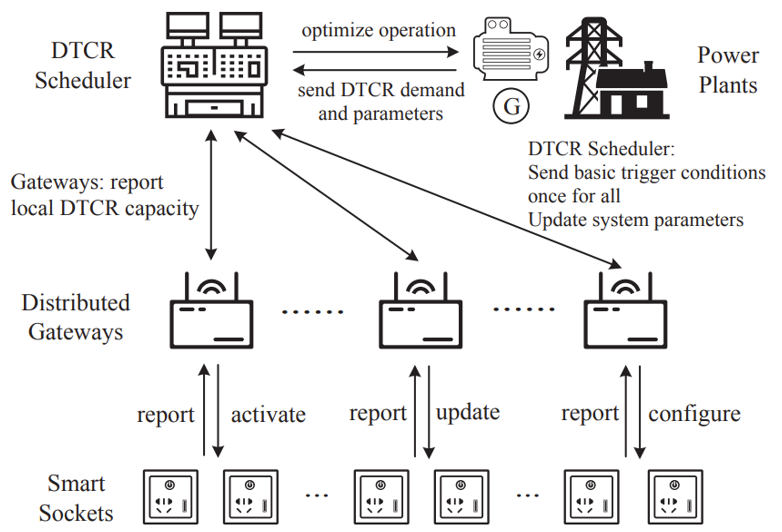
\includegraphics[scale=0.4]{figures/320341828_557303412943331_7871269242616177441_n.png}
    \caption{System design of decentralized transfer of contingency reserve \cite{Paper1Bottom-Up}}
    \label{2.2}
\end{figure}

\begin{figure} [H]
    \centering
    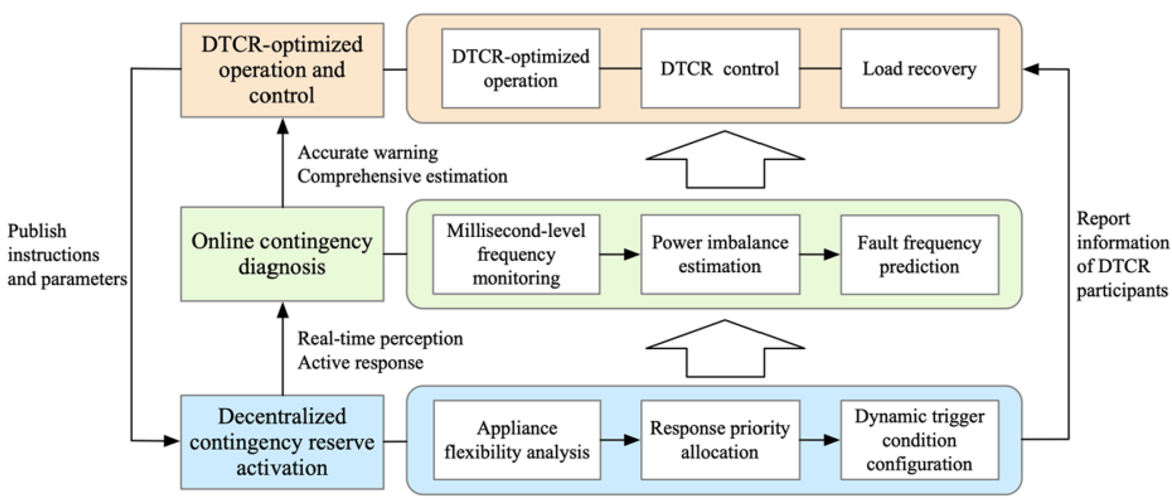
\includegraphics[scale=0.4]{figures/325098537_1216331305973113_1766856403111188462_n.png}
    \caption{Framework of decentralized transfer of contingency reserve\cite{Paper1Bottom-Up}}
    \label{2.3}
\end{figure}
From Figure \ref{2.2} and Figure \ref{2.3}, the decentralized transfer of contingency reserve (DTCR) method runs in distributed levels of optimal operation and control. When failure occurs in a specific section of the system, dispatch decisions can be done locally and the overall operation of the system remains unaffected. Compared to a centralized method of using load to provide contingency reserves, iterative exchange of large loads of information is not necessary through the proposed method and the use of smart sockets and distributed gateways. Since this bottom-up approach does not entirely depend on a central control center, the proposed method decentralizes the calculation burden of the system.

Another study \cite{Paper2Bottom-Up} under the bottom-up approach involves the aggregation of DERs and the concept of virtual powerplant is introduced to resolve the issue of the increasing number of DERs having time-varying states. This bottom-up approach is proposed to address the challenge of real-time flexibility in a large application.

\begin{figure} [H]
    \centering
    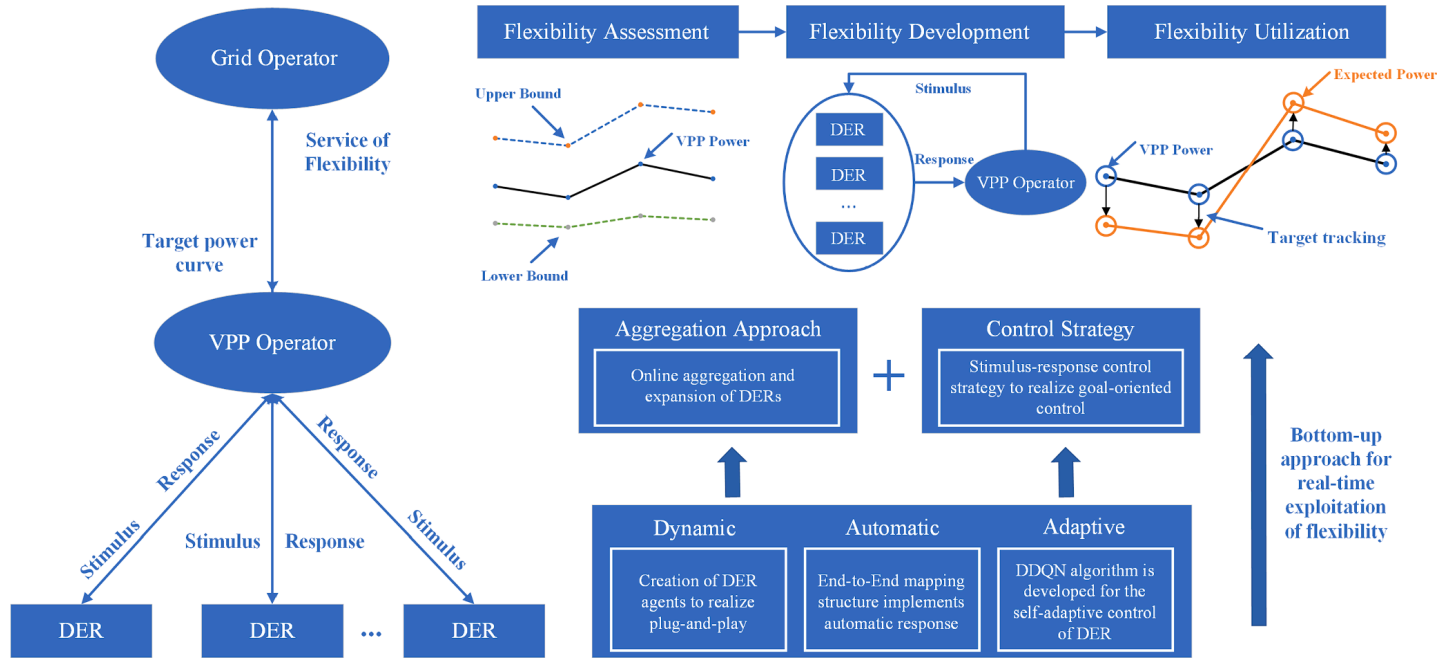
\includegraphics[scale=0.3]{figures/324502630_975795973391411_6414856379415667224_n.png}
    \caption{The scheme of dynamic exploitation of flexibility by VPP using bottom-up approach. \cite{Paper2Bottom-Up}}
    \label{2.4}
\end{figure}

From Figure \ref{2.4}, the DERs display the three essential characteristics of being dynamic, automatic, and adaptive. Compared to a centralized approach where all DERs heavily rely on a central control center, the proposed method increases the flexibility of DERs where the addition or removal of any DER will not affect the overall operation of the system and DERs can act automatically act on their own as their individual decision-making process do not have to rely on complete information from a central control unit. Moreover, DERs being autonomous can naturally adapt to the changing environment regardless of the different characteristics of DERs. 

Lastly, one study also applied the decentralization method
for Home energy management system (HEMS) for multiple homes with DERs \cite{Paper3Bottom-Up}. Most HEMS uses a centralized optimization method, but in this study, through a decentralized approach, it was able to reduce the computational complexity by distributing the centralized computation to decentralized entities that are capable of managing the energy consumption separately.

\begin{figure} [H]
    \centering
    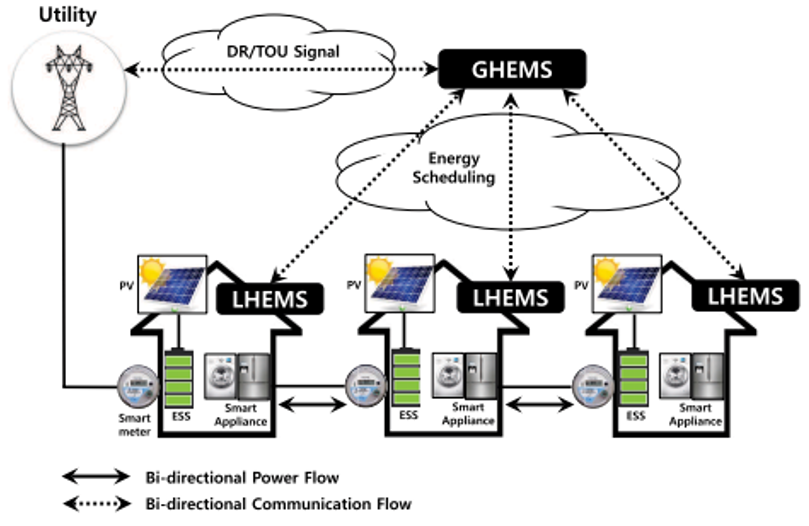
\includegraphics[scale=0.5]{319689493_2353696314795337_1096036110377907937_n}
    \caption{Conceptual architecture of the distributed HEMS (DHEMS).
 \cite{Paper3Bottom-Up}}
    \label{2.5}
\end{figure}

From the bottom-up approach shown in Figure \ref{2.5}, iterative communication between the two-level HEMS is not necessary which decreases the communication burden in the system. 

\section{Demand Response}
\label{section:sec02_02}

From the background of the study, it has been established that IDR programs are more suitable for large-scale demand-side management. To ensure the goal of IDR, it is essential to ensure accurate and fair DR performance evaluation, so that the customers can be compensated accurately.  Most IDR schemes use the CBL-based method to measure the contribution of DR participants.

\subsection{Customer Baseline Load (CBL)}

CBL is the forecasted load profile of a customer without a DR event as illustrated in Figure \ref{fig:CBL}.

\begin{figure} [H]
    \centering
    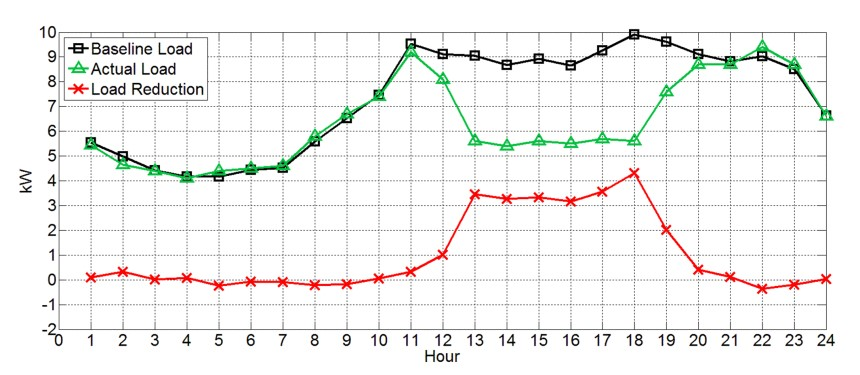
\includegraphics[scale=0.7]{figures/cbl.jpg}
    \caption{Illustration of CBL (black), resulting load after DR (green), and estimated load reduction (red) \cite{CBL}}
    \label{fig:CBL}
\end{figure}

As shown in Figure \ref{fig:CBL}, the load reduced by the DR participant (red) is the difference between the estimated CBL/baseline load (black) and the actual load of the customer during the DR event (green). There are several calculation methods used in estimating the CBL. Those methods were analyzed and tested by several studies to determine its accuracy. One of which is the study \cite{CBL}.

\begin{figure} [H]
    \centering
    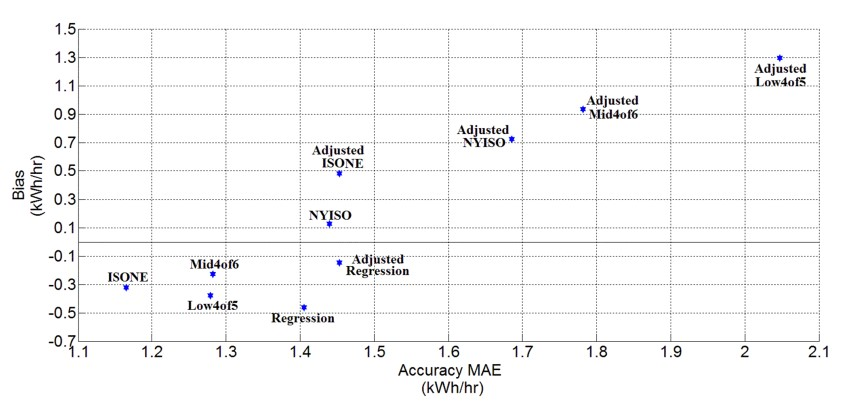
\includegraphics[scale=0.9]{figures/cbl_error.jpg}
    \caption{Mean absolute error and bias of different CBL calculation methods \cite{CBL}}
    \label{fig:CBL-error}
\end{figure}

Shown in Figure \ref{fig:CBL-error} is the result of their analysis which shows the different estimation methods and their accuracy and bias. The study states that no matter which method is adopted for estimating the CBL, a large amount of end-user data collection, storage, and computation are all significant challenges if CBL is to be calculated in a centralized form. The results of the case study performed shows that the inaccuracy of the CBL calculation methods causes the hypothetical utility of the case study to pay at least half of its revenue on the event day as rebate. The CBL-based method leads to a random distribution of the utility's revenue as a reward for the false load reduction.

\subsection{Coupon Incentive-based Demand Response}

Aside from the estimation errors of CBL, there are problems in existing IDR programs that uses CBL-based methods. In the IDR scheme from \cite{CIDR}, load serving entities (LSEs) could offer retail customers coupon incentives via near-real-time information networks to induce demand response for a future period in anticipation of intermittent generation ramping and/or price spikes. 

\begin{figure} [H]
    \centering
    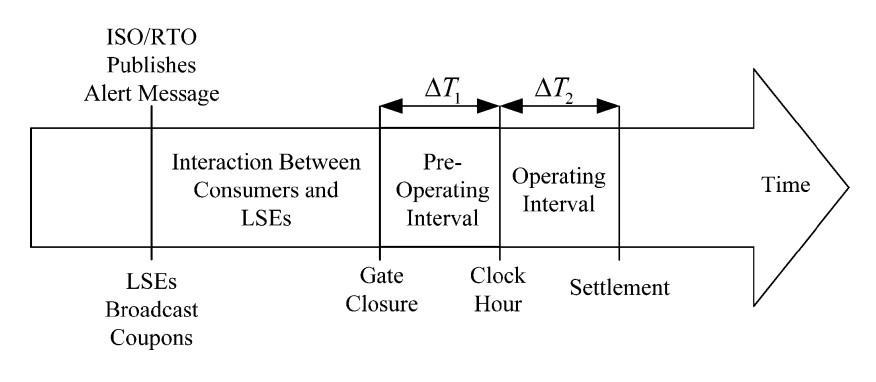
\includegraphics[scale=0.8]{EEE Documentation/figures/cidr.jpg}
    \caption{Timeline for CIDR implementation \cite{CIDR}}
    \label{fig:S11_graph}
\end{figure}

The ISO/RTO alerts the LSE to call for demand response. Then, the LSE will broadcast coupons for DR participants. Several communication iterations will be done between the LSE and the participants until the gate closure and the demand response is organized for dispatch. The settlement for the incentive is done after the operating interval. 

With this, the scheme offers flexibility to customers because it is voluntary unlike direct load control, and there is high consumer surplus because the coupons can have different rates unlike the classical IDR with just a flat rate. However, this scheme computes for the CBL in a centralized manner hence the LSE needs to process a large amount of data. Furthermore, it requires multi-round communication iterations which causes increased communication burden and a hindrance to large-scale implementation. Lastly, there is increased response uncertainty because it is voluntary.

\subsection{Coupon-based Demand Response - A Strategic Bidding Model for Load Serving Entities}

The study \cite{IDR-2} proposes a scheme with a strategic bidding approach for LSEs in deploying a Coupon-based demand response with consideration of wind power uncertainties and customer’s behavior patterns toward different coupon prices.

\begin{figure} [H]
    \centering
    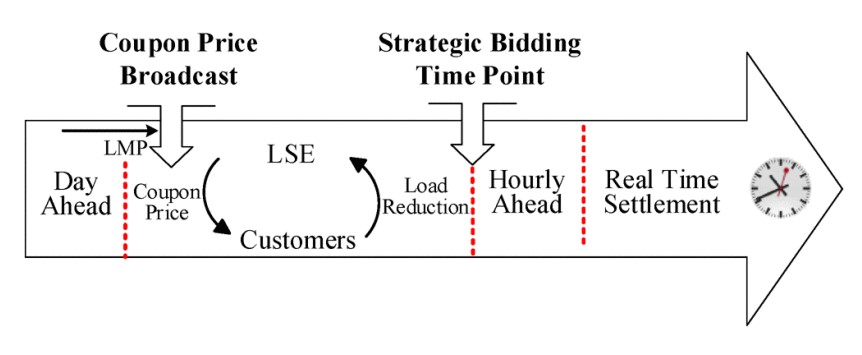
\includegraphics[scale=0.7]{figures/idr2.jpg}
    \caption{Timeline for strategic bidding \cite{IDR-2}}
    \label{fig:S11_graph}
\end{figure}

Unlike the previous, the coupon prices will be broadcasted a day ahead then that’s when the settlement between the LSE and customer occurs. Then there is an additional bidding point at an hour ahead where customers can bid prices for their additional load reduction. This addresses the problem of increased communication burden and system uncertainty, however; the scheme still computes for the individual CBLs centrally which is a hindrance to its large-scale application.

\cleardoublepage{}

\section{Decentralized Systems for Demand Response}
\label{section:sec03_03}

Because of using CBL-based methods, most Incentive-based DR programs are not suitable for large-scale applications as it would require large data collection, heavy data processing, and complex computation. Hence, decentralized schemes for demand response are explored.

\subsection{Customer Directrix Load (CDL)-based DR}

To solve the issue of scalability and unfair incentive measurement,  Customer directrix load (CDL)-based demand response is proposed in \cite{CDL} where CDL is used to replace the CBL. The CDL is defined as the desired load profile for the flexible loads of each DR customer.

\begin{figure} [H]
    \centering
    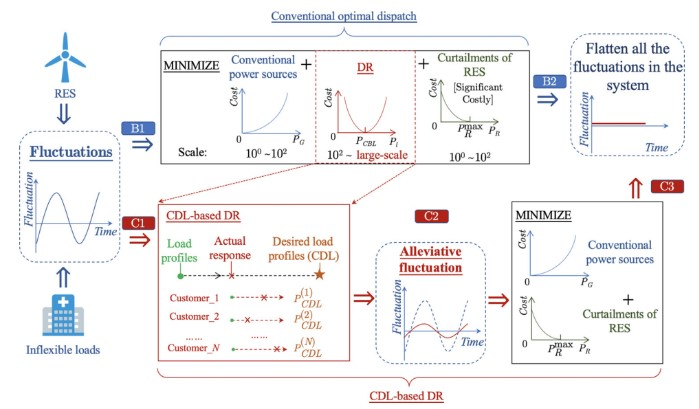
\includegraphics[scale=0.9]{figures/cdl2.jpg}
    \caption{Relationship between the conventional optimal dispatch and CDL-based method \cite{CDL}}
    \label{fig:cdl2}
\end{figure}

Shown in Figure \ref{fig:cdl2} is the comparison between the conventional optimal dispatch and the CDL-based demand response. Conventionally, the optimal dispatch is formulated as an optimization problem that aims to minimize the costs of all controllable sources. This is illustrated in B1 and B2 of Figure \ref{fig:cdl2}. To solve the problem of this scheme, the CDL-based DR decouples the DR event from the complex optimization problem as shown in C1, C2, and C3. 

\begin{figure} [H]
    \centering
    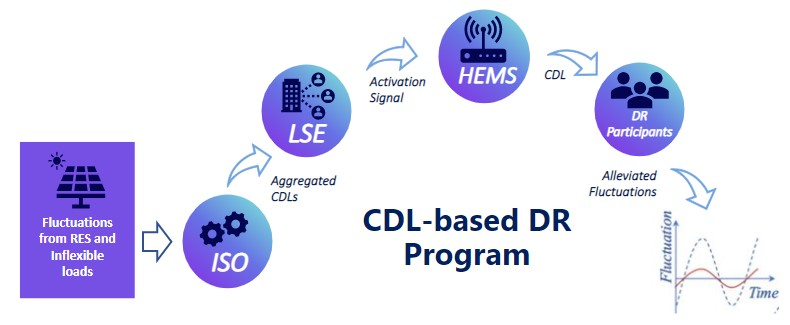
\includegraphics[scale=0.9]{figures/cdl.jpg}
    \caption{General flow of the CDL-based demand response}
    \label{fig:cdl-methodo}
\end{figure}

Shown in Figure \ref{fig:cdl-methodo} is the general flow of the CDL-based DR. The input to the scheme is the real-time states of the power system, while considering the renewable energy output and inflexible loads at a given time. From the anticipated power imbalances, the Independent service operator (ISO) computes for the ACDL, an aggregated form of the CDLs which is the desired load profile needed to compensate for the fluctuations at the system level given by the formula:

\begin{equation}
  \Delta P_{ACDL}=(P^{max}_{R}(t)-P^{max}_{R}(t-1))-\Delta P_{C}(t) \label{ACDL}
\end{equation}

where \(P^{max}_{R}(t)\) is the maximum available RES output at time t, and \(P_{C}(t)\) is the total power of inflexible loads at time t.

The ACDL will then be transmitted to the Load Serving Entity (LSE) in which it will compute an activation signal which is a ratio of the change of the ACDL between two timeframes given by:

\begin{equation}
  \Delta r(t)=\frac{ P_{ACDL}(t)- P_{ACDL}(t-1)}{ P_{ACDL}(t-1)} \label{CDLr}
\end{equation}

This activation signal will then be transmitted to the home energy management systems (HEMS) of each DR participant to compute for the CDL individually:
\begin{equation}
    \ P_{CDL}^i(t) = (1+r(t))P_{CDL}^i(t-1) \label{PCDL}
\end{equation}

where \(P_{CDL}^{i}(t)\) is the CDL for customer i at time t. The CDL reflects the load curve the customer needs to follow for the given time slot. Given this, the DR participants will set their consumption preference through the HEMS and they will be compensated through electric bill discounts based on how near their flexible load consumption is to the CDL. The incentive function is defined as:

\begin{equation}
    \ f_{d}(d^{i}) = D_{0}e^{-\frac{d^{i}}{\sigma}}\label{incentive}
\end{equation}

where \(f_{d}\) is the incentive function, which is the same for all customers. \(D_{0}  \epsilon  (0,1]\) is the maximum rate a customer can receive, \(\sigma\) is control coefficient that will be set by the discount provider, and \(d^{i}\) is the mean squared error between the actual load curve and the CDL.

After the DR event, the fluctuations of the system will be alleviated and will be further flattened using either conventional power sources or curtailment of RES. Shown in Figure \ref{fig:acdl} is an example illustration of ACDL and CDL curves.

\begin{figure} [H]
    \centering
    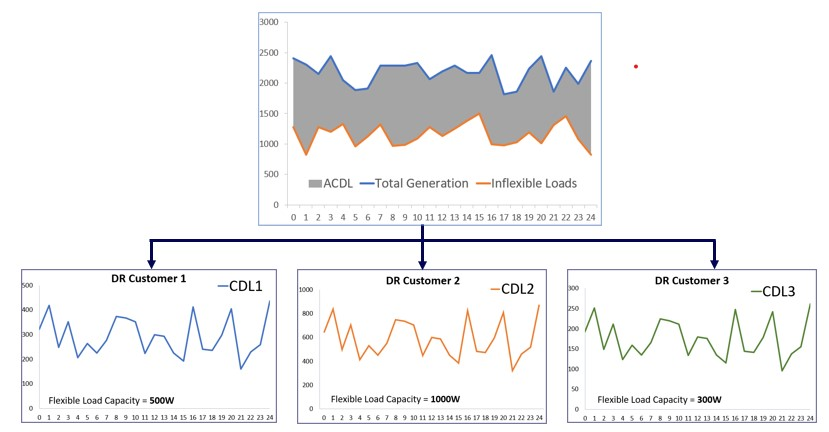
\includegraphics[scale=0.7]{figures/acdl-cdl.jpg}
    \caption{Illustration of ACDL and CDLs }
    \label{fig:acdl}
\end{figure}

Although the CDL-based DR results to a more accurate DR performance measurement, fair load allocation, and decentralized computation, this scheme is rather a dogmatic way of implementing DR. The required responses from participants may seem infeasible because the computed CDLs are based on just the registered maximum capacity of flexible load at all time intervals, regardless of the comfort level of customers at certain time intervals. Further, in a well-designed electrical grid, power imbalances are small. Hence, the computed CDLs would be small since the imbalance  will be divided among a  large number of participants. This renders DR participants unable to respond since they can only respond in realistic discrete intervals.

\section{Summary}
The advantages and disadvantages of the two methods mentioned before are presented in Table 2.1. The traditional Top-Down approach is shown to be prone to several issues in its communication system due to being heavily dependent on a centralized control system that increases the complexity on the computation and decision-making process of DERs. To address these limitations, a bottom-up approach allows the distribution of tasks and computation that decreases the communication burden of the system. Moreover, Table 2.2 shows how a CDL-Based DR Program is able to resolve the issue of scalability and unfair incentive measurement. However, this scheme does not consider the customer's comfort level and how much possible control they have on their load consumption.

\begin{longtable}[c]{| c | c |}
 \caption{Top-Down and Bottom-Up Comparison Table\label{long}}\\
 \hline
 Top-Down & Bottom-Up\\
 \hline
 \endfirsthead
 \hline
 \multicolumn{2}{|c|}{Continuation of Table \ref{long}}\\
 \hline
 Top-Down & Bottom-Up\\
 \hline
 \endhead
 \hline
 \endfoot
 \hline
 \endlastfoot
\makecell{- dependent on a centralized control system}  & \makecell{- the decision-making process of DERs \\ is not fully dependent on the control system}\\ 

 \makecell{-increases computational complexity\\ on the central control system.\\}
 & - distributed computation\\

\makecell{- the system suffers from sub-optimal solutions\\ when the communication system is down.} & - increases flexibility of DERs \\

 \end{longtable}

 \begin{longtable}[c]{| c | c |}
 \caption{CDL-Based DR Program Pros and Cons\label{long}}\\
 \hline
Pros & Cons\\
 \hline
 \endfirsthead
 \hline
 \multicolumn{2}{|c|}{Continuation of Table \ref{long}}\\
 \hline
 Pros & Cons\\
 \hline
 \endhead
 \hline
 \endfoot
 \hline
 \endlastfoot
\makecell{- decentralized computation} & 
\makecell{- physical and comfort levels of customers are not considered}\\
\hline
\makecell{- fair load allocation} & 
\makecell{- requested responses from participants may seem \\ infeasible as participants can only
respond in discrete levels}\\
\hline
\makecell{- accurate DR performance \\measurement} &
\makecell{- requested responses become too small for participants\\ to realistically respond to. (This is especially prevalent\\ in large-scale systems where the ACDL is divided into several\\ amounting to hundreds-thousands of participants.)\\}

 \end{longtable}


As summarized above, this leads to the decision to use a bottom-up approach in the study's proposed scheme to address the scalability issues mentioned. Also, an improved design of the existing CDL scheme is proposed for a more feasible way for DR participants to comply at all time intervals. 


\cleardoublepage{}

\chapter{Problem Statement and Objectives \label{cha:ProbStatement}}
\section{Problem Statement} \label{sec: Problem}

The traditional centralized approach used in large-scale applications is prone to issues by being heavily dependent on a centralized control system that increases computational complexity and the system may suffer from sub-optimal solutions when the communication system is down. Due to the limitations mentioned, there are still scalability problems that need to be addressed in the implementation of demand response programs. With this, studies about decentralized schemes are explored such as the CDL-based scheme for fairer incentive measurement in large applications.  However, CDL employs a dogmatic way of implementing a DR program wherein the LSEs dictate how much a customer should be consuming, regardless of the customer’s comfort level.

\section{Objectives of the Project}
\label{section:sec_obj}

The objectives of this study is to implement a demand response (DR) scheme that is suitable for large-scale demand-side management (DSM), and uses a fair, and accurate DR measurement to ensure profit for both customers and suppliers. The detailed objectives are shown below:

\begin{enumerate}
\item Propose a DR framework using customer-directrix response (CDR)-based methods for large-scale demand-side management (DSM),
\item Conduct case studies by varying the number of DR participants and consumers,
\item Discuss the performance of the scheme in terms of load curves and accuracy of incentive allocation, and;
\item Analyze the effectiveness of the proposed DR scheme using the final peak load reductions.
\end{enumerate}

\section{Scopes and Limitations}
\label{scopes}
The study will only focus on the performance of the CDR-based method and will not investigate the fairness of the scheme. Fairness in this study's context refers to the ability of two similar consumers being given equal opportunities in their participation in their scheme, this was investigated in \cite{CDL} and since the proposed scheme is heavily influenced by the CDL, CDR is assumed to be fair. This however will neither be investigated or proven. Further, the study will only be purely theoretical and will not be physically implemented. 
\cleardoublepage{}

\chapter{Methodology}\label{cha:Methodology}

In this chapter, the framework for Customer Directrix Response (CDR) is explained which aims to address the issues mentioned in the previous chapters.  The methodology is composed of the overview, data gathering, mathematical formulation, program development, program verification, and simulations.

\section{Overview} \label{Overview}

 For a general overview, the proposed scheme is built upon the existing scheme, CDL-based DR. In this scheme, the DR participants are informed on how much they should increase or decrease their consumption rather than informing the participants on what load profile their flexible loads need to follow. The CDR scheme primarily addresses the scalability problem and the infeasible requests of the CDL-based DR as explained in section \ref{2.4} by allowing the participants to pool the responses requested from them and have the most appropriate participant/s among them to respond. With this, the scheme is called Customer Directrix Response (CDR) scheme. Figure \ref{fig:top-level} shows an overview of the proposed scheme.

\begin{figure} [H]
    \centering
    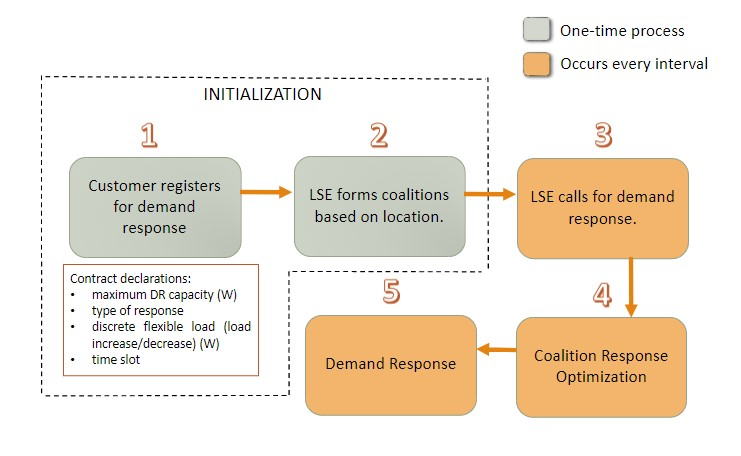
\includegraphics[scale=1]{figures/top-level.jpg}
    \caption{Top-level CDR scheme flowchart}
    \label{fig:top-level}
\end{figure}

The scheme starts with the registration of the customers for demand response where they will declare the necessary information needed which will be explained in section \ref{subsec: contract}. After obtaining information about the participants, the LSE forms coalitions based on the location of the participants. The motivation for the coalition protocol will be further explained in section \ref{sssec: framework}. After this initialization stage, the LSE can now call for demand response. Coalition Response Optimization will be done and the participant/s chosen to respond will be dispatched for demand response.




\subsection{Contract Declarations}\label{subsec: contract}
Upon registration for the DR program, participants are required to declare the following:

\begin{enumerate}
    \item Maximum Demand Response Capacity (in W) - maximum power the customer can use for demand response in a day; determines how much response is requested from the participant per time interval
    \item Response Type - load increase/load reduction/load shift
    \item Discrete flexible load (in W) - the amount of load the customer can increase/decrease/shift per interval 
    \item Time Slot - the preferred time slot of demand response the customer wishes to participate in\\
    (i.e. Customer 1 who have a maximum DR capacity of 1000W registers 100W discrete load decrease from 9am to 2pm)
\end{enumerate}

Comparing the scheme to the CDL-based DR
, both are decentralized as participants compute for their own response, accurate as the DR events are based on real time states of the system, and fair as there is fair load allocation and participants cannot take advantage of the system to gain unwarranted incentives.


For their difference, DR participants in the CDR scheme, unlike the CDL, are given the prescribed load increase or decrease needed for a time period instead of the load profile for the flexible load of the customer. To show that, here is an example plot for the ACDL and the ACDR. Furthermore, unlike CDL, the CDR scheme allows participants to form coalitions to improve their overall demand response which will discussed more in section \ref{subsec: coalition}.

\begin{figure} [H]
    \centering
    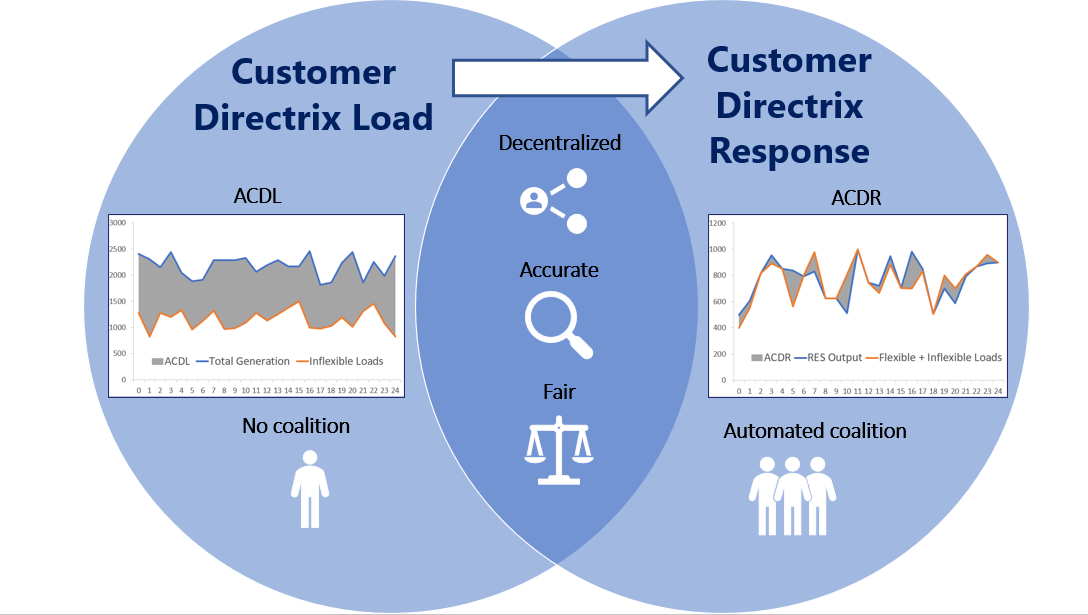
\includegraphics[scale=0.5]{figures/Differences.png}
    \caption{Difference between CDL and CDR }
    \label{fig:Differences}
\end{figure}



\section{Data Gathering} \label{sec: Gather}
\subsection{Data Sets}\label{subsec: sets}
Three main types of data sets were used in testing the CDR algorithm. The main difference of each data set from one another is its number of DR participants. Namely 50, 5000, 10000, and 16000 participants. 

The 50, 5000, and 10000,  participants data sets were simply used to test the performance of the algorithm in different sizes of an electrical grid. 

While the 16000 participants data set was extensively used to test the robustness, performance, and behavior of the algorithm in different scenarios. Hence, the 16000 participants data set consisted of several sub types which will we be discussed in detail in \cite{}.

To ensure that each data set has variability on its loads, the magnitudes and load trends from participant to participant were varied. Each participant follows a daily residential load curve but no two participants have equal load trend magnitudes. The different load curve trends are seen in the images below:\par

\begin{figure}[h]%
    \centering
    \subfloat[\centering Load Curve 1 \cite{}]{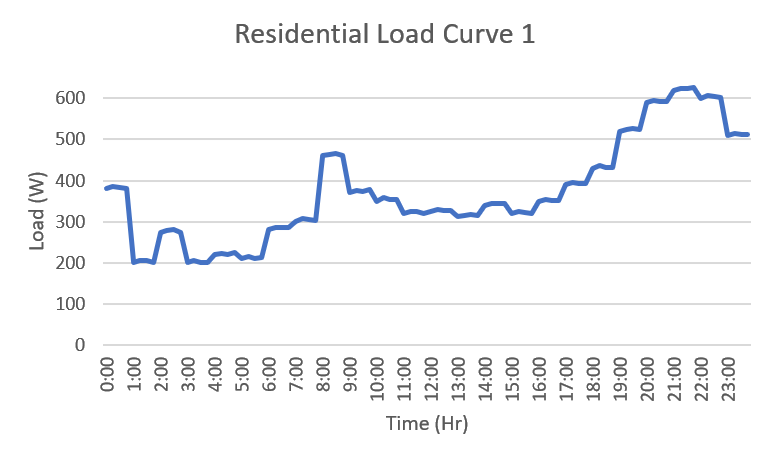
\includegraphics[width=7cm]{R1.png}}%
    \qquad
    \subfloat [\centering Load Curve 2 \cite{}]
    {{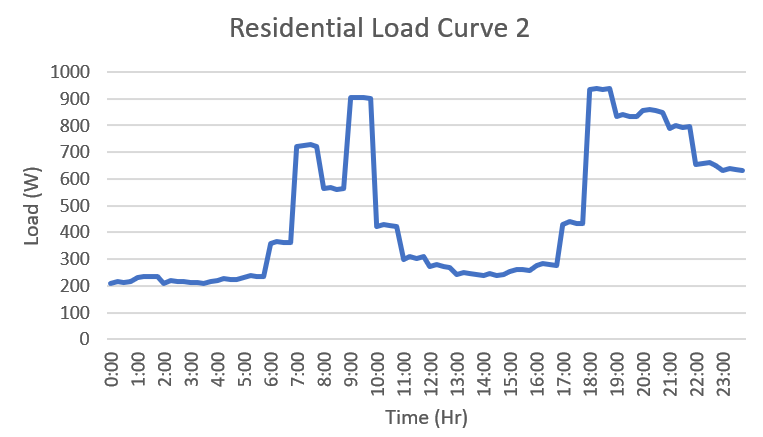
\includegraphics[width=7cm]{R2.png} }}%
    \label{fig:example}%
\end{figure}

\begin{figure}[h]%
    \centering
    \subfloat [\centering Load Curve 3]
    {{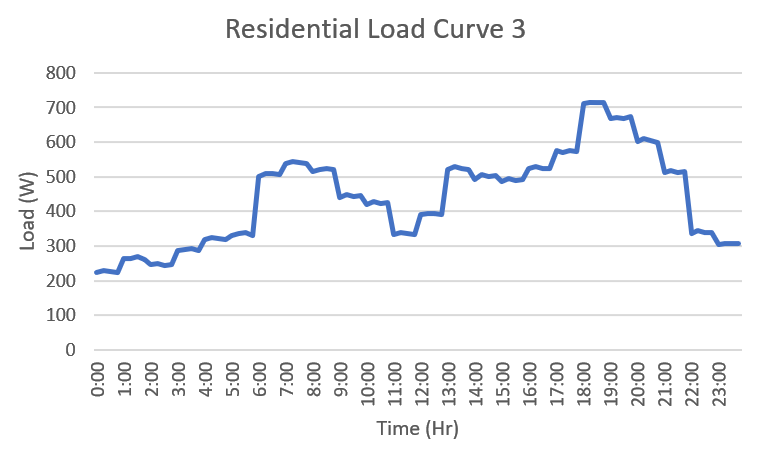
\includegraphics[width=7cm]{R3.png} }}%
    \qquad
    \subfloat [\centering Load Curve 4 ]
    {{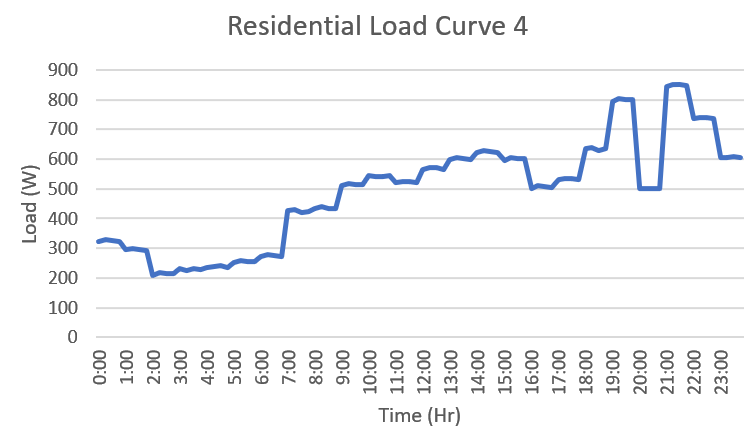
\includegraphics[width=7cm]{R4.png} }}%
    \label{fig:example}%
\end{figure}

\begin{figure}[h]%
    \centering
    \subfloat[\centering Load Curve 5 ]
    {{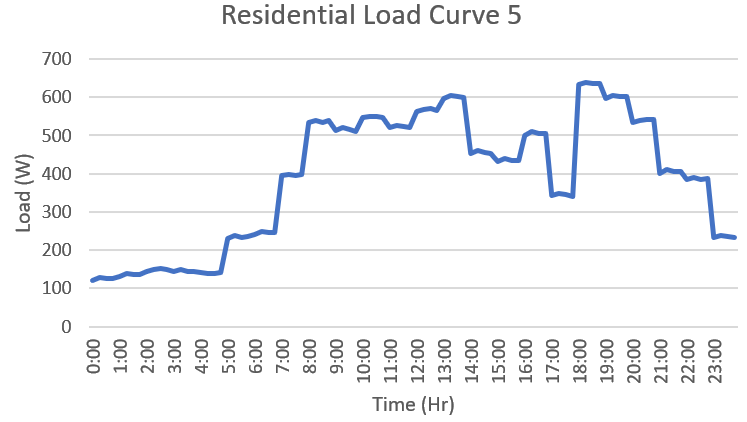
\includegraphics[width=7cm]{R5.png} }}%
    \qquad
    \subfloat[\centering Load Curve 6 ]
    {{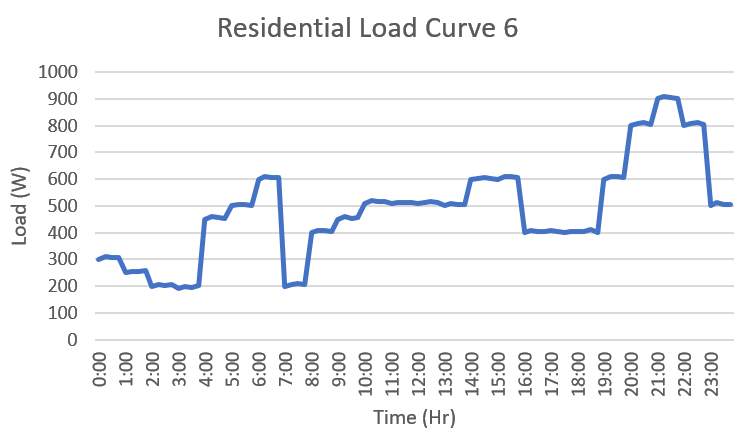
\includegraphics[width=7cm]{R6.png} }}%
    \label{fig:example}%
\end{figure}

\begin{figure}%
    \centering
    \subfloat [\centering Load Curve 7 ]
    {{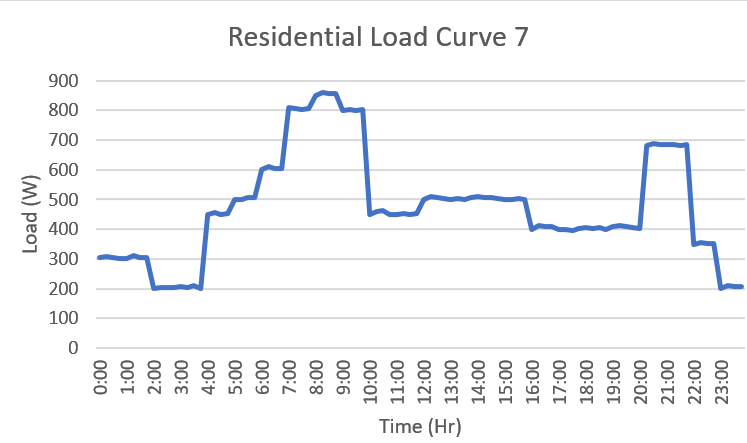
\includegraphics[width=7cm]{R7.png} }}%
    \qquad
    \subfloat [\centering Load Curve 8 ]
    {{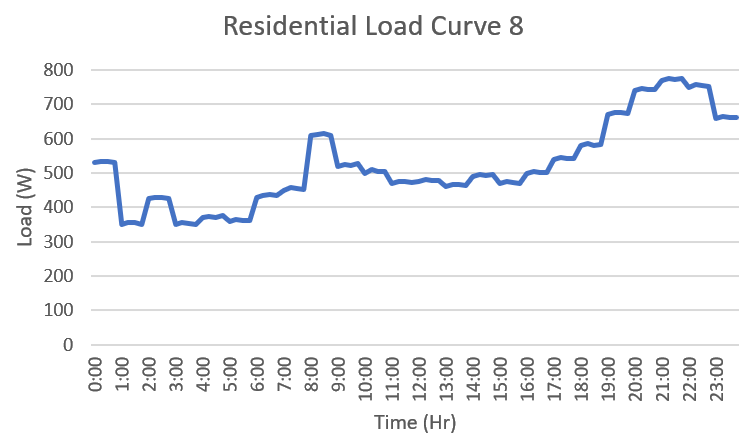
\includegraphics[width=7cm]{R8.png} }}%
    \label{fig:example}%
\end{figure}

\begin{figure}%
    \centering
    \subfloat[\centering Load Curve 9 ]
    {{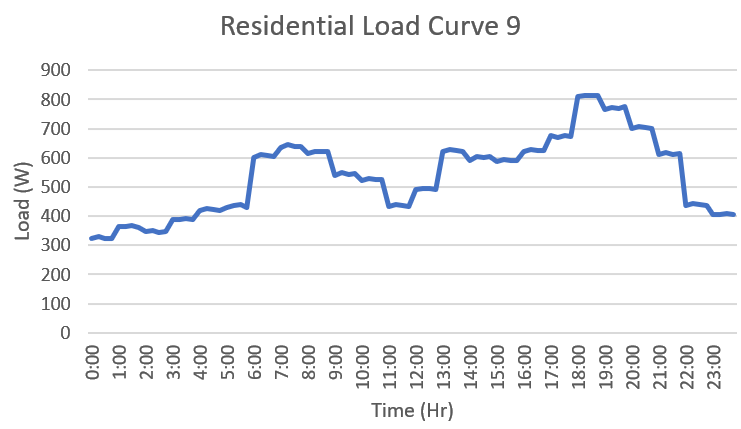
\includegraphics[width=7cm]{R9.png} }}%
    \qquad
    \subfloat [\centering Load Curve 10 ]
    {{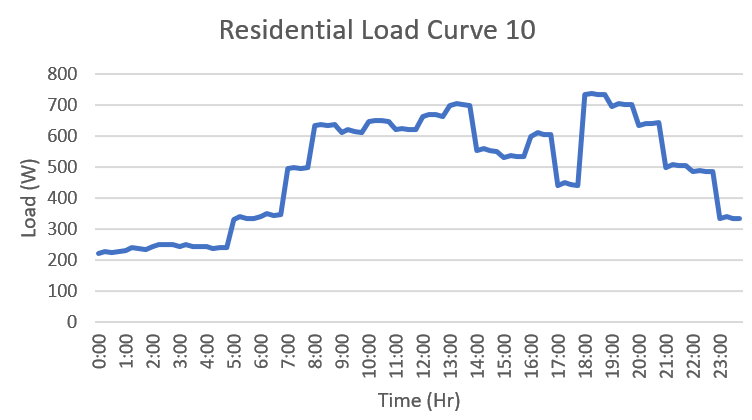
\includegraphics[width=7cm]{R10.png} }}%
    \label{fig:example}%
\end{figure}



\subsubsection{50 Participants}\label{subsubsec: 50parti}
The 50 participants data set contains 5 locations on where each location has 10 participants. Moreover, the distribution of grid imbalances, participant discrete responses are normally distributed with a mean of zero (0). While all participants can participate in all time intervals (i.e. no declared time slots)

\subsubsection{5,000 Participants}\label{subsubsec: 5000parti}
The 5,000 participants data set contains 50 locations on where each location has 100 participants. Moreover, the distribution of grid imbalances, participant discrete responses are normally distributed with a mean of zero (0). While all participants can participate in all time intervals (i.e. no declared time slots)

\subsubsection{10,000 Participants}\label{subsubsec: 10000parti}
The 10,000 participants data set contains 500 locations on where each location has 20 participants. Moreover, the distribution of grid imbalances, participant discrete responses are normally distributed with a mean of zero (0). While all participants can participate in all time intervals (i.e. no declared time slots)

The different characteristics of the aforementioned data sets are listed in the table below.



\begin{table}[]
\begin{adjustbox}{width=1\textwidth}
\small
\begin{tabular}{|c|c|c|c|c|c|}
\hline
\textbf{Data Set} & \textbf{Number of Coalitions} & \textbf{Number of Participants per Coalition} & \textbf{Distribution of Grid Imbalances} & \textbf{Distribution of Participants Discrete Response} & \textbf{Declared Time Slots} \\ \hline
50                & 5                             & 10                                            & Normally Distributed  ($\mu$ = 0)             & Normally Distributed ($\mu$ = 0)                           & None                         \\ \hline
5,000             & 50                            & 100                                           & Normally Distributed  ($\mu$ = 0)             & Normally Distributed  ($\mu$ = 0)                           & None                         \\ \hline
10,000            & 500                           & 20                                            & Normally Distributed  ($\mu$ = 0)             & Normally Distributed ($\mu$ = 0)                           & None                         \\ \hline
\end{tabular}
\end{adjustbox}
\caption{Basic Data Sets Summary} 
\end{table}





The different compositions are listed   below:

\begin{enumerate}
\item 80\% of participants are only able to increase their load consumption while 20\% of participants are only able to decrease their load consumption,
\item  80\% of participants are only able to decrease their load consumption while 20\% of participants are only able to increase their load consumption,
\item  50\% of participants are only able to increase their load consumption while 50\% of participants are only able to decrease their load consumption,
\item  100\% of participants are only able to increase their load consumption,
\item 100\% of participants are only able to decrease their load consumption,
\end{enumerate}

Moreover, this data set has 3 versions based on its load-generation imbalances. The different versions are as follows:

\begin{enumerate}
\item  is skewed towards a lack of power generation, 
\item  is skewed towards a lack of load consumption,
\item  no skew, the load imbalances are normally distributed
\end{enumerate}

The histogram of the imbalances of the different versions are shown in the images below:

\begin{figure} [H]
    \centering
    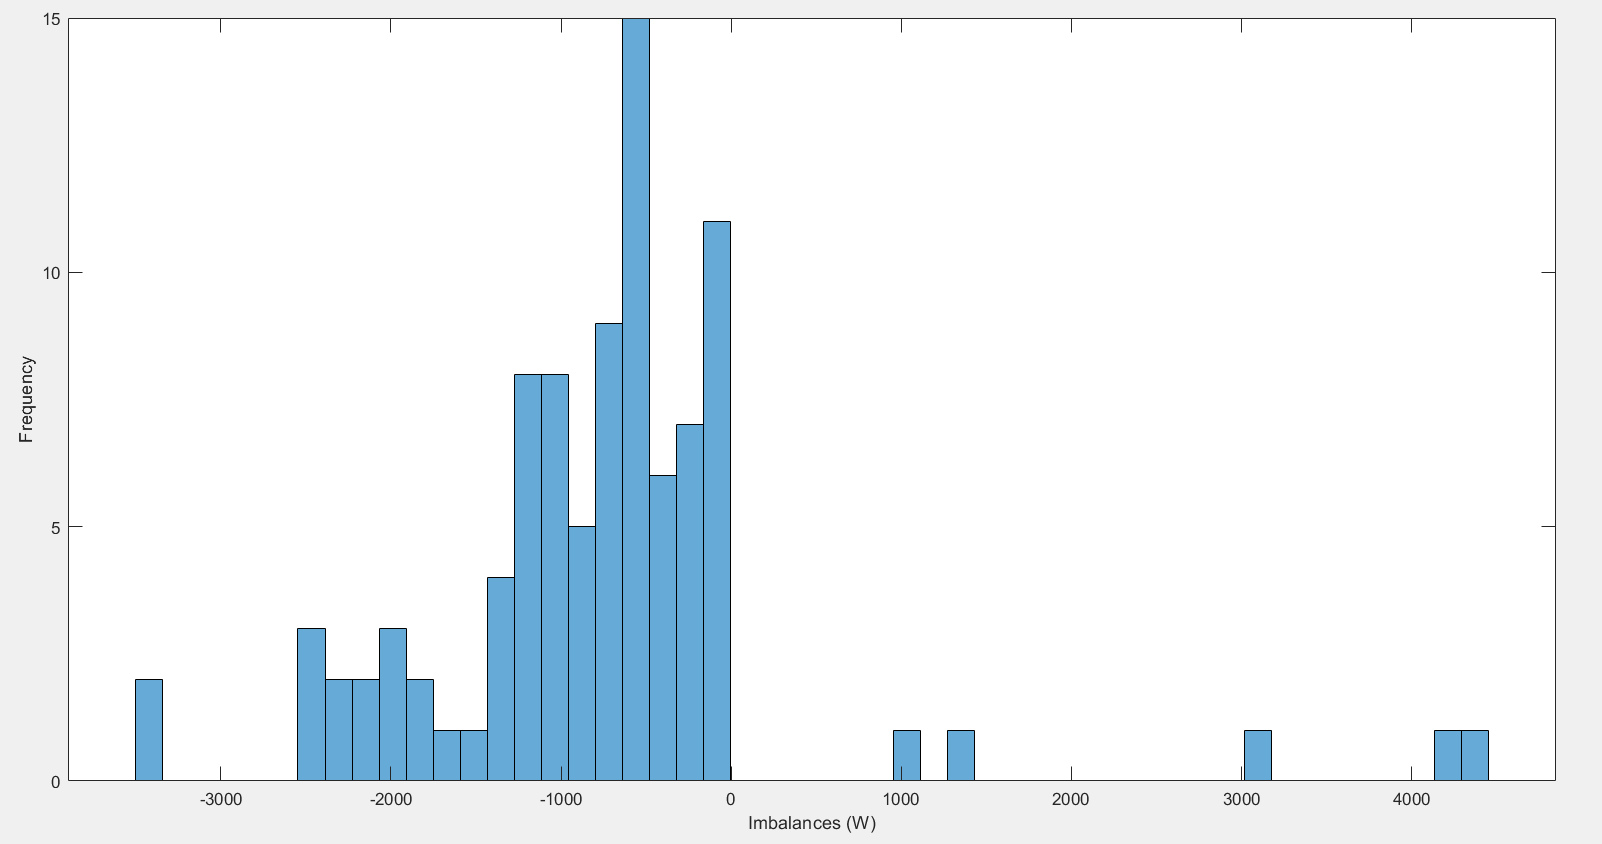
\includegraphics[scale=0.3]{L.png}
    \caption{Case 1. Skewed towards a lack of power generation}
    \label{fig:Differences}
\end{figure}

\begin{figure} [H]
    \centering
    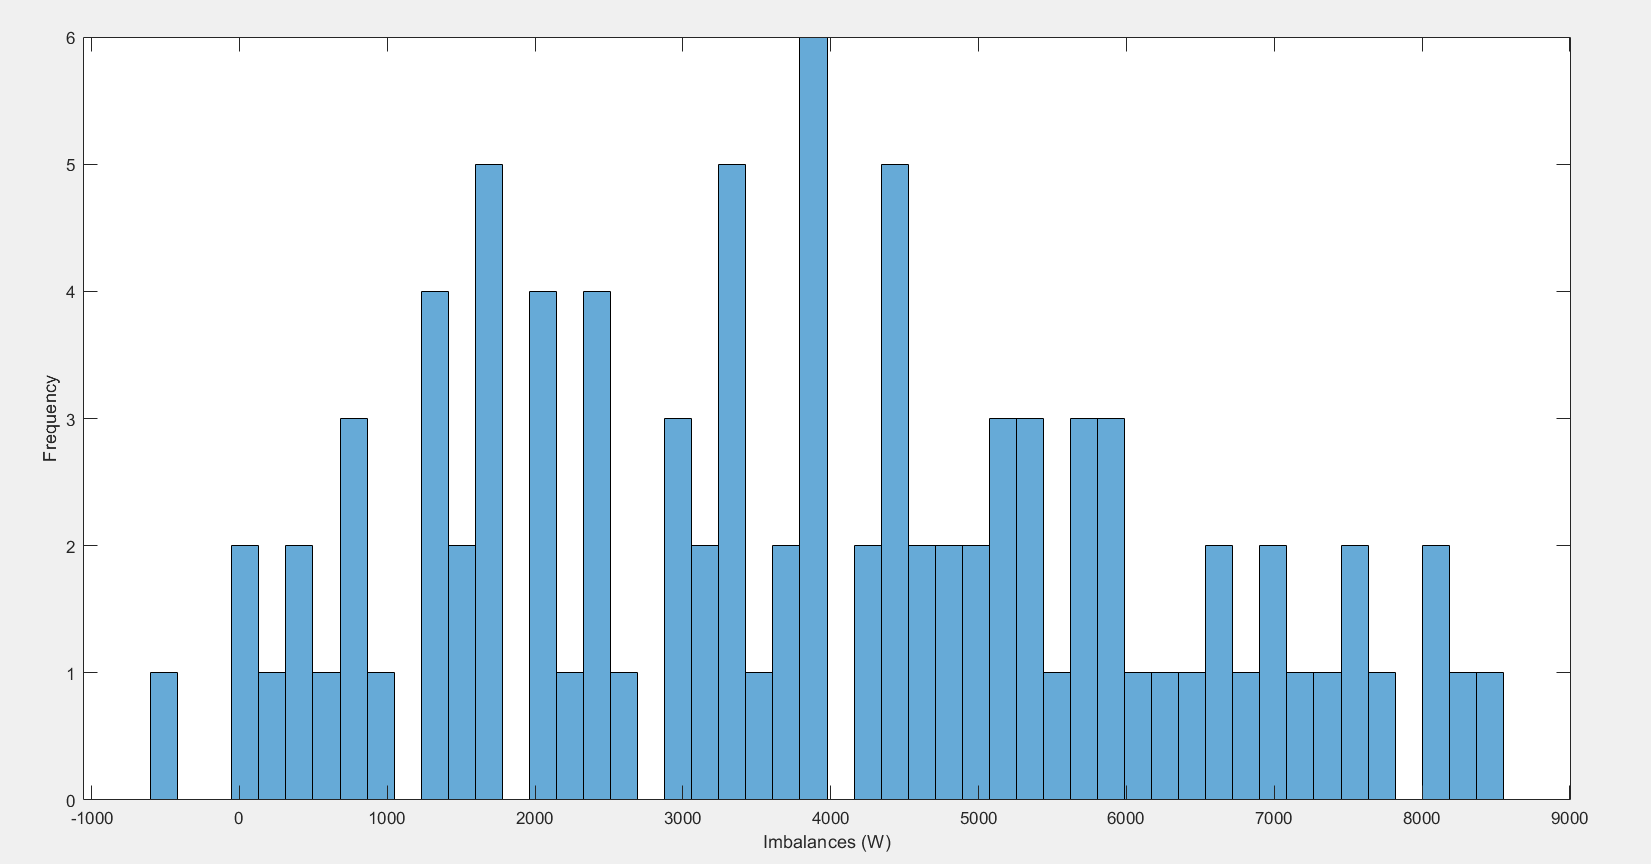
\includegraphics[scale=0.3]{R.png}
    \caption{Case 2. Skewed towards a lack of load consumption}
    \label{fig:Differences}
\end{figure}

\begin{figure} [H]
    \centering
    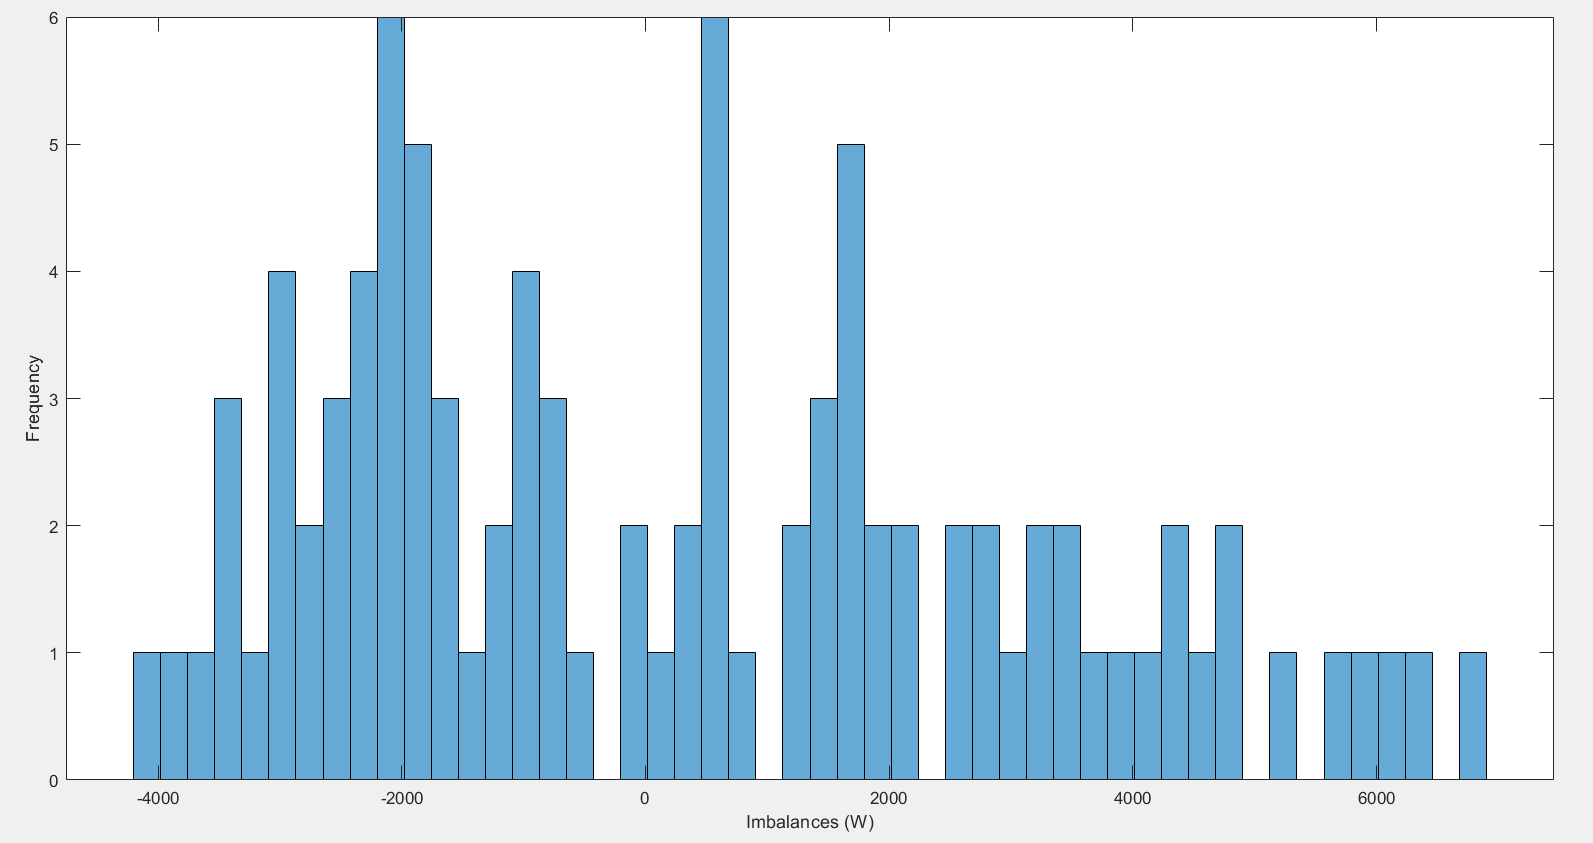
\includegraphics[scale=0.3]{N.png}
    \caption{Case 3. No Skew}
    \label{fig:Differences}
\end{figure}




\subsection{User-Defined Performance}\label{subsec: performance}


\section{Theoretical Framework and Mathematical Formulation} \label{sec: Math}

Equations for the algorithm to function properly were defined in the succeeding section. Most equations were derived from the previous proposed CDL scheme. The CDR-based Demand Response Framework as mention in section \ref{Overview} heavily relies on its ability to group a grid's participants into different coalitions in an effort to alleviate a grid's imbalances. However, for a coalition to properly respond to the imbalances of the grid different variables needs to be established, computed or dispatched first. A quick overview of the algorithm is presented below:
\begin{enumerate}
\item  System level imbalances are quantified by the ISO as the ACDR, 
\item  The ACDR is transmitted to the LSE wherein the activation signal is computed,
\item  The activation signal is then transmitted to all participants.
\item  The activation signal will dictate the requested response for a given participant, this is known as its CDR. The participants of a given coalition will then pool their CDRs
\item The most appropriate participant based on the pooled CDR and their declared discrete response capability will then be determined by the parent HEMS.
\item The parent HEMS will then send a dispatch signal to the most appropriate daughter HEMS. Wherein that participant will then respond.
\item Step 5 will then repeat until no participant is able to respond or the pooled CDR is fully satisfied.
\end{enumerate}
A more fully detailed explanation of each step is presented in the succeeding sections. While a visualization of the algorithm's framework is shown in figure \ref{fig:Overview of CDR Scheme}.

\begin{figure} [H]
    \centering
    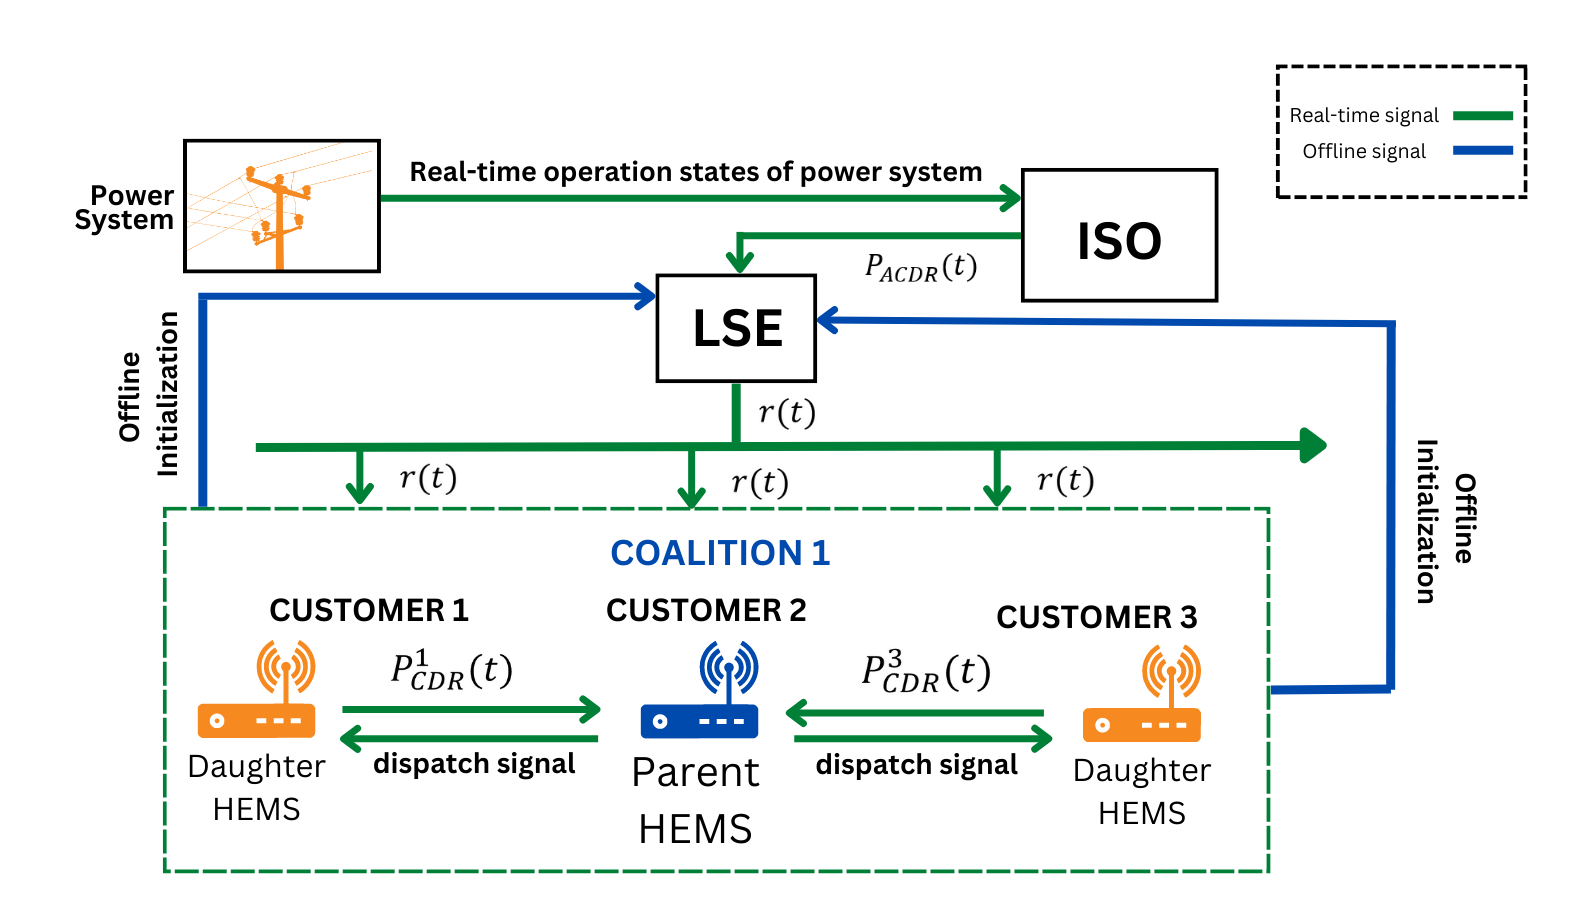
\includegraphics[scale=0.45]{figures/dr_framework.png}
    \caption{Overview of CDR Scheme}
    \label{fig:Overview of CDR Scheme}
\end{figure}
 paper proposes to deploy the scheme with a coalition feature wherein DR participants can autonomously form coalitions to help each other comply with their own respective CDRs. The need for coalitions was realized since it was acknowledge that:

\begin{itemize}
    \item The need to consider the comfort of DR participants especially during humid conditions where consumers may not want to curtail their consumption. The adjustable offering capacity as discussed in section \ref{subsec: performance}, contributes to this point.
    \item Coalitions may help DR participants increase their received incentives as coalitions will allow them to follow their respective CDRs much more accurately.
    \item Since DR participants will be able to follow their CDRs more accurately this will help in maintaining the power balance of the grid.
\end{itemize}
\subsubsection{Framework} \label{sssec: framework}

The framework of the coalition system is shown in figure \ref{fig: Coalition Framework}. DR participants will participate in Bi-directional communication within the designated radius to determine which participants they will form coalitions with, determined by their respective offers. After which the participants will divert or receive power with the ones in their coalition

\begin{figure} [H]
    \centering
    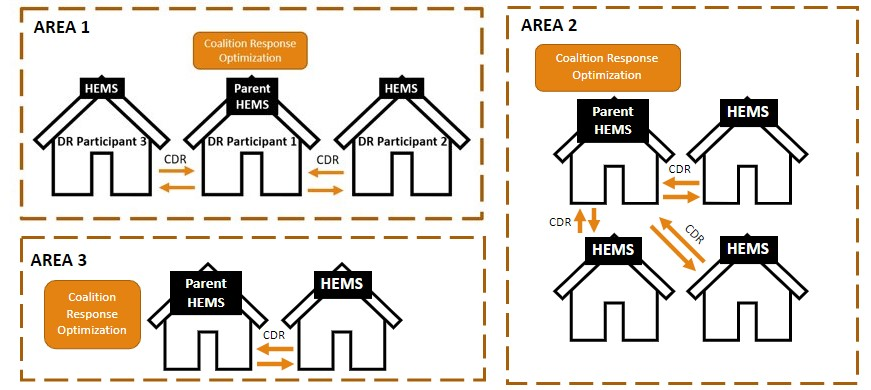
\includegraphics[scale=0.9]{figures/area.jpg}
    \caption{Coalition Framework}
    \label{fig: Coalition Framework}
\end{figure}

\subsection{Aggregated Customer Directrix Response} \label{subsec: ACDR}

 The Aggregated CDR (ACDR) is defined as the desired load reduction/increase at the system level that can offset all the fluctuations.  It will borrow most concepts from the CDL scheme with significant differences, which was discussed in Section \ref{Overview}. First and most significant difference is that the CDR will no longer dictate a DR participant on how much it should be consuming at a certain given time but rather it will now advise the participants on how much they should increase or decrease their consumption. 


With that being said, the ACDR can be obtained by solving the simple power balancing equation:
\begin{equation}
P_G(t) + P_{Res}(t)=P_D(t)+P_C(t)\label{eqn: Balancing}
\end{equation}

Where \(P_G(t),P_{Res}(t),P_D(t),P_C(t)\) are the total power of conventional
power sources, RES, DR customers, and inflexible loads in the entire
system at time t, respectively. 

As the CDR-scheme also aims to have the maximum possible renewable energy source integration total power of conventional power sources will not be considered in the calculation of the ACDR thus; 

\begin{equation}
P_{Res}(t)=P_D(t)+P_C(t)\label{eqn: derive 1}
\end{equation}

Then finding the difference between two time slots:

\begin{equation}
\Delta P_{Res}(t)=\Delta P_D(t)+\Delta P_C(t)\label{eqn: derive 2}
\end{equation}

Then from the definition of the ACDR let  \(\Delta P_D(t) = P_{ACDR}(t)\) then rearranging the equation the ACDR equation is then:

\begin{equation}
 P_{ACDR}(t)=\Delta P_{Res}(t)-\Delta P_{load}(t)\label{eqn: ACDR}
\end{equation}

 \(\Delta P_{RES}(t) \) and \(P_{load}(t)\) Which will be taken by the ISO, and when the ISO detects a fluctuation, it will call for a DR Event. Do take note that this happens an hour ahead before the DR event.  

\subsection{Activation Signal} \label{subsec: r}

After the ISO computes for the ACDR it will transmit it to the LSE where it will compute for the activation signal. The activation signal is simply a changing ratio where it facilitates the equal division of the ACDR among the DR participants. Mathematically defining the activation signal:

\begin{equation}
r(t)=\frac{ P_{ACDR,2}(t)- P_{ACDR,1}(t)}{ P_{ACDR,1}(t)}\label{eqn: activation}
\end{equation}

where:
\begin{equation}
P_{ACDR,2}(t) = (P_R(t)+P_R(t-1))-(P_C(t)+P_C(t-1)) \label{eqn: ACDR 2}
\end{equation}

\begin{equation}
P_{ACDR,1}(t) = (P_R(t-1)+P_R(t-2))-(P_C(t-1)+P_C(t-2))\label{eqn: ACDR 1}
\end{equation}


\subsection{Customer Directrix Response}\label{subsec: CDR}

This activation signal will then be transmitted to individual DR Participants wherein their own respective Home energy management system (HEMS) will compute for their CDR. The HEMS will then take a snapshot of the current consumption \(P_b(t)\)  and compute for its CDR. The CDR can be computed using the equation \ref{eqn: CDR}. 

\begin{equation}
 P_{CDR}^i(t) = (1+r(t))P_{CDR}^i(t-1) \label{eqn: CDR}
\end{equation}

As the current CDR is dependent with the previous CDR an initial CDR must be initialize. In this light when a DR participant registers for the CDR-scheme they are required by the LSE to declare their maximum flexible load capacity in which will be used in computing for the initial CDR. This can be easily computed using equation \ref{eqn:initial CDR}.


\begin{equation}
 P_{CDR}^i(t-1) = \frac{S^i_{max}}{\sum_{i=1} S^i_{max}}P_{ACDR}(t-1) \label{eqn:initial CDR}
\end{equation}

Where \(S^i_{max}\) is the maximum flexible capacity of Customer i. 


\subsection{Coalition Protocol} \label{subsec: coalition}
After the HEMS computes for its CDR, it will then send its CDR to it's coalition's designated Parent HEMS. This is true for all Daughter HEMS of a coalition. The Parent HEMS will then pool all the CDR it has received, where it will be referred to as the Total CDR (TCDR) of a coalition. From here the Parent HEMS will choose the most appropriate participant among its coalition to respond. The conditions to determine the most appropriate participant will be discussed in the succeeding section.

\subsubsection{Coalition Response Optimization} \label{sssec: conditions}

As mentioned in blank the Parent HEMS has knowledge of  the discrete flexible load, response types and the time slots of its participants. In this light the following are the conditions or criteria of the Parent HEMS to determine the most appropriate participant to respond for its coalition.

    \begin{itemize}
\item \textbf{The participant with the discrete response that decreases the imbalance most -} This refers to the discrete response that will reproduce the smallest difference among all the discrete response of the coalition. Mathematically this can be quantified as:
\begin{equation}
Participant_{res} = min(Difference)
\end{equation}
\begin{equation}
Difference =[d_1, d_2, d_3, ...,d_i ]
\end{equation}
\begin{equation}
d_i = |R_i|-|TCDR|
\end{equation}
     Where \(i, R_i, Participant_{res}\) is the participant number,  the discrete flexible response of customer \(i\) and the most appropriate participant to respond according to this condition.

\item \textbf{Its discrete response's sign must match the TCDR's. A positive discrete response will only respond to a positive TCDR and vice versa -} There will be cases wherein a certain participant will produce the smallest \(d\) while having the it having a discrete response opposite of the TCDR. If such a participant responds this will only worsen the imbalance of the grid.
\item \textbf{The participant responding must not worsen the imbalance of the system after responding. -} This will ensure that the participant responding will not worsen the imbalance even if it satisfies the 1st and 2nd conditions. Mathematically a participant can respond if it satisfies the condition below:
\begin{equation}
|d_i| < |TCDR|
\end{equation}
    \end{itemize}
\begin{itemize}

\end{itemize}

Once a participant is deemed appropriate the TCDR will then be updated by subtracting it to the participant's discrete flexible response.
\begin{equation}
TCDR_{updated} = TCDR - R_{i}
\end{equation}
Once a new TCDR is computed the Paren HEMS will continue to find the next appropriate participant to respond. This will continue until TCDR reaches 0 or no participant is deemed appropriate to respond.

\subsection{Summary}\label{sssec: Summary}
For a short summary the real time states of the power system, specifically the change in load and the RES Generation,\(\Delta P_{LOAD}\)  and \(\Delta P_{RES}\) will be taken by the ISO.

The ISO will then calculate the Aggregated CDR using equation\ref{eqn: ACDR} , The ACDR will then be transmitted to the LSE where it will compute for the activation signal using equation \ref{eqn: activation}.

The activation signal will then be transmitted to all DR Participants through their own respective HEMS, once the HEMS receives the activation signal it will immediately compute for its CDR using equation \ref{eqn: CDR} . All daughter HEMS of a coalition will then submit its CDR to its coalition's parent HEMS. Once the Parent HEMS receives the CDRs of its co-coalition members, it will then start to determine the most appropriate participant to respond by checking the conditions discussed in section\ref{sssec: conditions}. This will step will repeat until the TCDR is depleted or no participant can longer appropriately respond.


\begin{figure} [H]
    \centering
    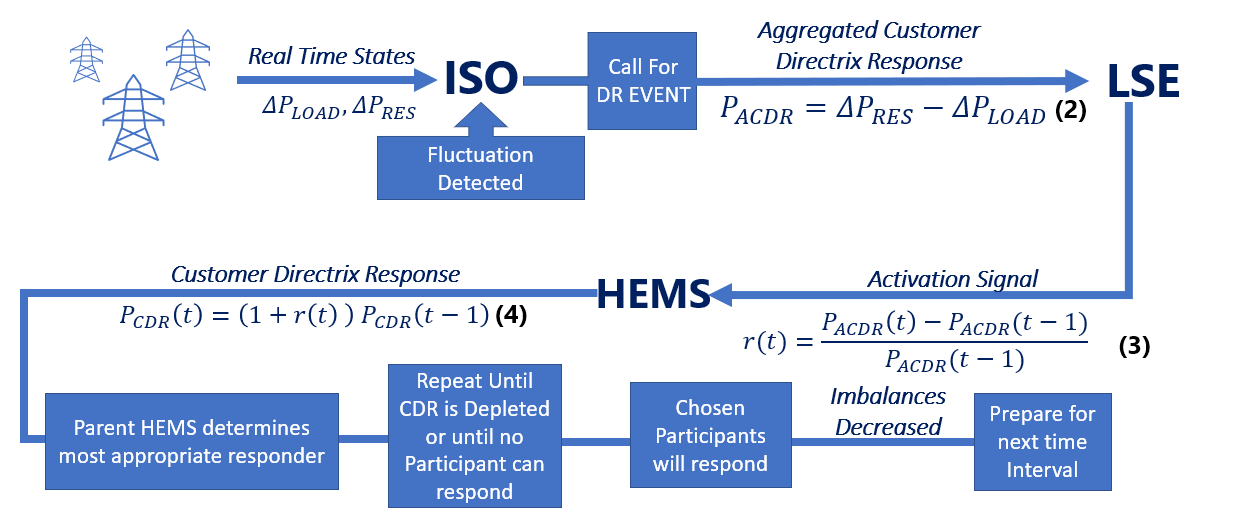
\includegraphics[scale=0.6]{figures/Summary_CDR.png}
    \caption{CDR Scheme Summary}
    \label{fig:CDR Scheme}
\end{figure}


\section{Program Development} \label{sec: PD}

MATLAB will serve as the primary programming environment for this study. With that being said 5 main programs were identified to ensure that the proposed CDR Scheme will work as intended namely an ACDR program, Activation Signal program, CDR program, Coalition program and Incentive program.  Each program will be generating its own outputs. The flow and the outputs and inputs of the mentioned programs are shown in figure \ref{fig: Program Development Flowchart}. The Res Generation curve, and the  Load Curves will be inputted into the ACDR program which will produce the ACDR. The ACDR will then be inputted into the activation signal program which will produce the activation signal. Then additional inputs will be needed specifically the Maximum Flexible load capacity and the Upper and limits lower limits. This together with the activation signal will then be inputted into the CDR program. Which will produce the CDR and the offers. Which will be the basis if whether coalitions will be formed. Lastly the incentives will be computed. 

 

\begin{figure} [H]
    \centering
    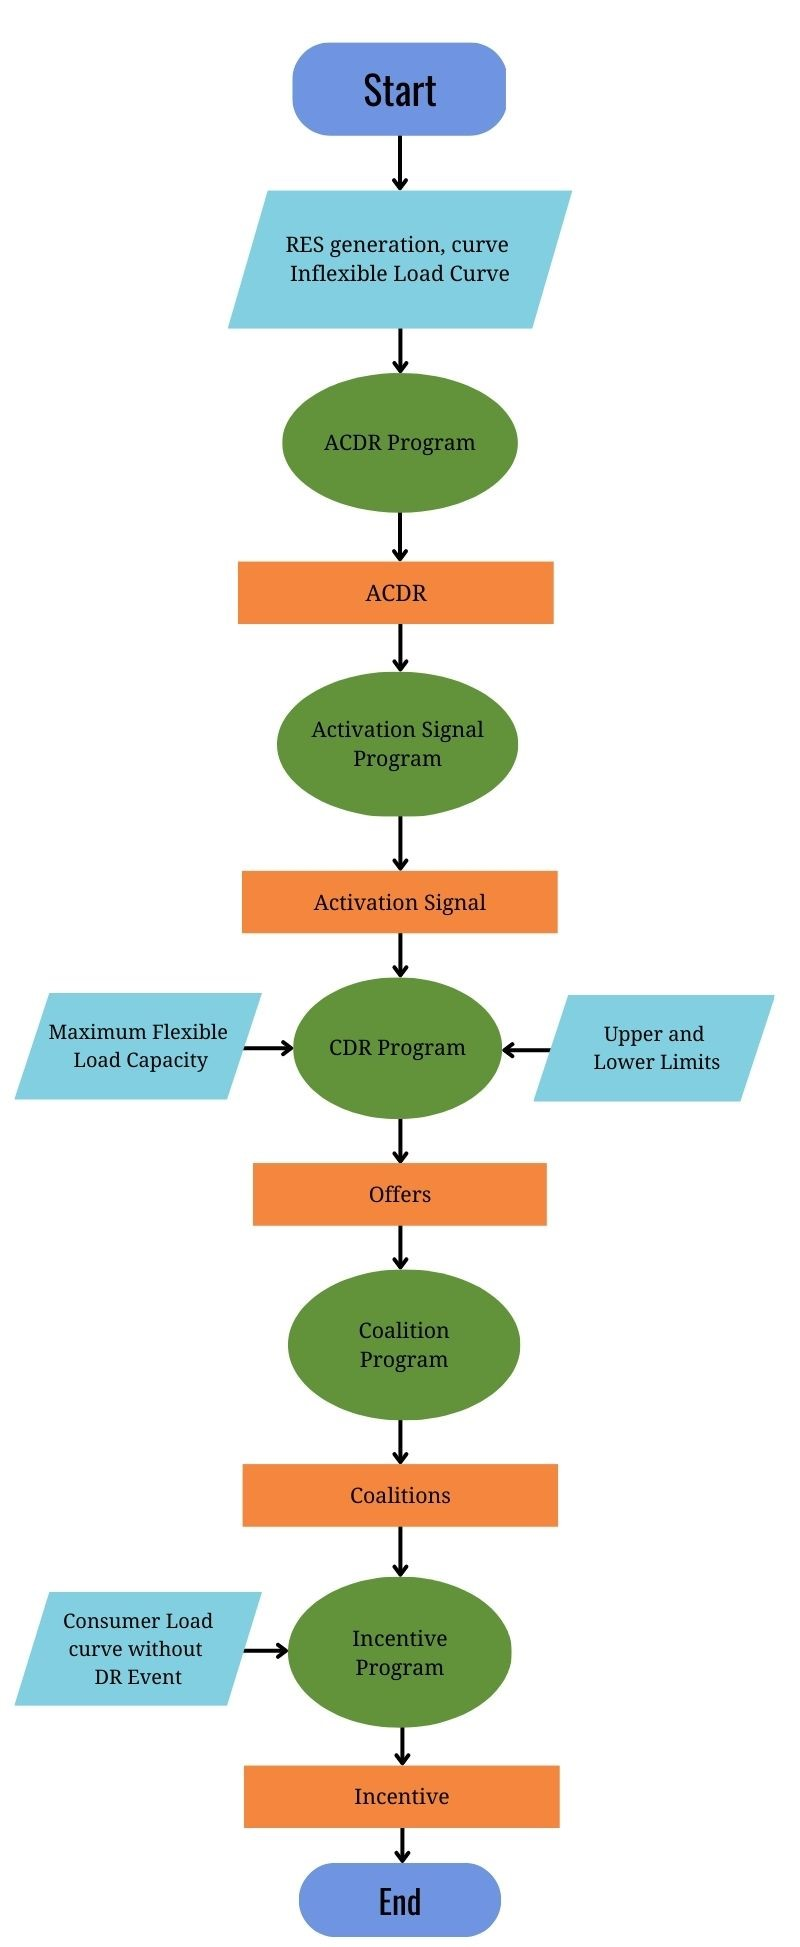
\includegraphics[scale=0.42]{figures/Program.jpg}
    \caption{Top-Level Program}
    \label{fig: Program Development Flowchart}
\end{figure}

\subsection{Coalition Algorithm} \label{sssec: Coalition Algorithm}
The automated coalition program at customer-level is shown in Figure  \ref{fig: Coalition Algorithm}.Alpha is first checked,  then an offer is put up. The offer will then be used to determine the offer.Once a coalition is formed, alpha is overwritten. When the overwritten alpha is 0 the coalition scheme ends if not, it will continue to find other participants to form coalition with. 

\begin{figure} [H]
    \centering
    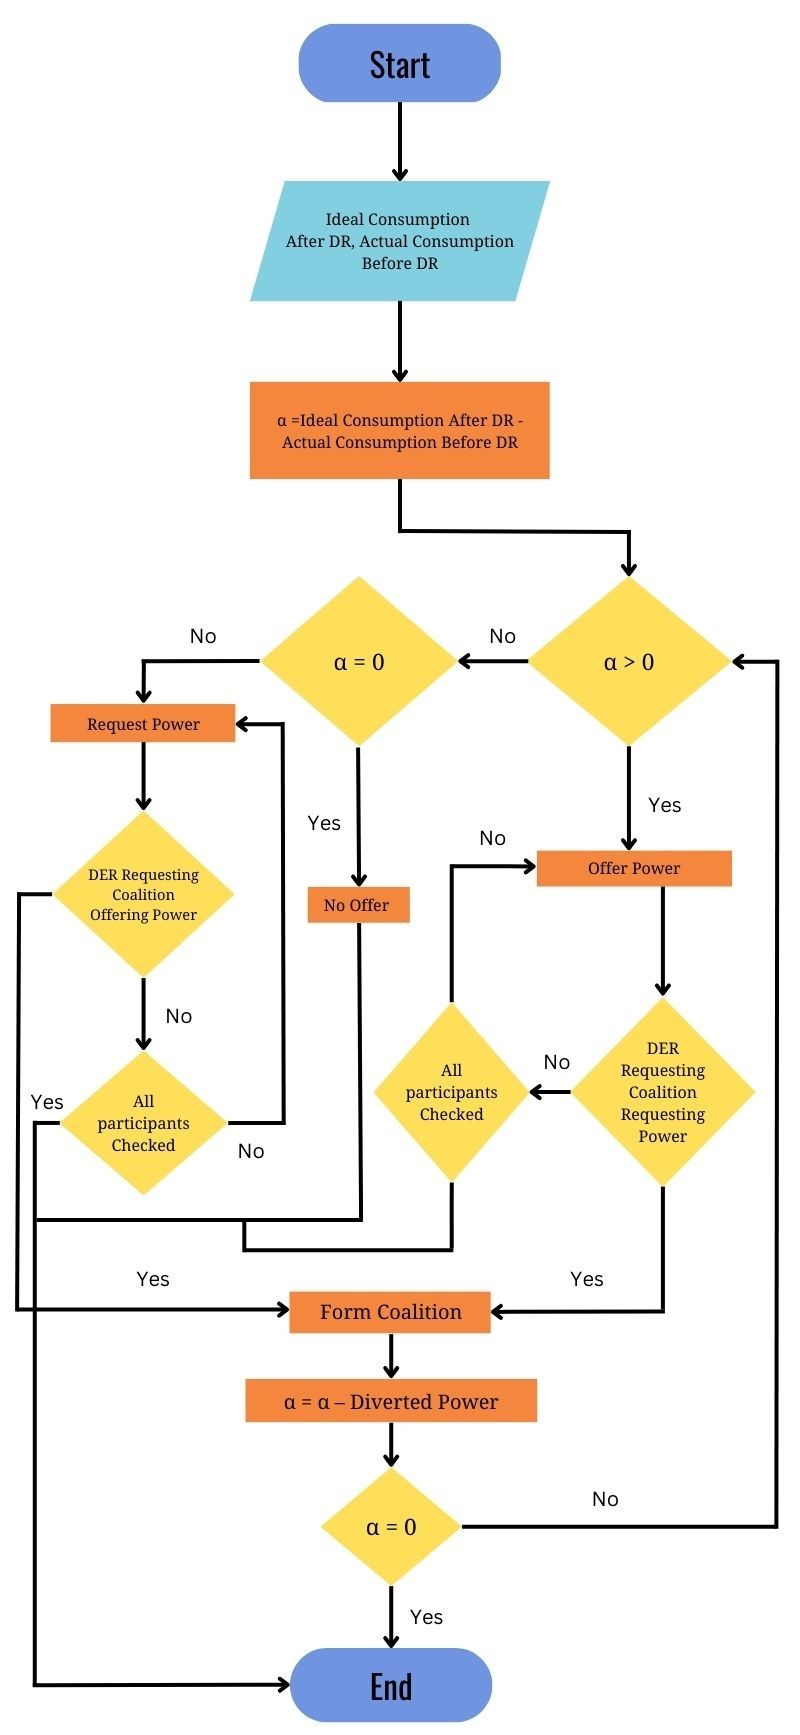
\includegraphics[scale=0.42]{figures/Specific Coalition.jpg}
    \caption{Automated Coalition Program per Customer}
    \label{fig: Coalition Algorithm}
\end{figure}

\section{Program Verification} \label{sec: PV}

To verify the accuracy and correctness of the program, the data set will be divided into 40 subsets where each subset will contain 5 participants. This will allow the program to cycle through different data subsets in the course of the verification. The program must be able to in all subsets:

\begin{enumerate}
    \item The aggregated demand response of participants follow the trend of the ACDR.
    \item Reduce the mean square error between the supply and load after the DR event.
    \item Individual demand responses must only respond within their designated limits.
\end{enumerate}

Debugging will be done if necessary.

\cleardoublepage{}

\section{Simulations} \label{sec: Sims}

To analyze the performance of the CDR framework in alleviating the system imbalances, case studies are performed to determine the factors that have a significant effect on the system performance. The variables analyzed are the following:
\begin{enumerate}
    \item number of coalitions
    \item distribution of imbalances throughout the day
    \item distribution of discrete responses
    \item width of time slots
    \item amount of discrete responses relative to the grid imbalance
    \item distribution of time slots
    \item coalition response composition
\end{enumerate}

\subsection{Case 1: Varying the number of coalitions} \label{Case1}
Given a constant amount of system imbalance, the fulfillment of demand response may change depending on the number of coalitions in the system. To investigate this, five simulations with varying numbers of coalitions were done using MATLAB. In order to make inferences about the result, other variables are maintained constant.

\subsection{Case 2: Varying the distribution of imbalances throughout the day} \label{Case2}
In typical systems, bulk of the imbalances are concentrated during peak periods. To investigate the effect of this, the peak periods are changed by changing the distribution of the imbalances throughout the day. A skewed to the left distribution results in more negative imbalances which consequently requires more load reduction while a skewed to the right distribution results in more positive imbalances which consequently requires more load increase responses.

\subsection{Case 3: Varying the distribution of discrete responses} \label{Case3}
Since the LSE can ask for a load increase or load decrease depending on the system  imbalance, the DR performance depends on the type of response (load increase/load reduction) and capacity of the discrete responses of the participants. With this, the distribution of the discrete responses of the participants are varied by changing its skewness. 

\subsection{Case 4: Varying the width of the time slots} \label{Case4}
The declared time slot defines when the participant will be actively participating in the demand response. Given this, the effect of time slots is investigated by changing the duration of the time slots for all participants. 

\subsection{Case 5: Total amount of discrete responses relative to the total system imbalance} \label{Case4}


\chapter{Preliminary Findings\label{cha:Prelims}}

A case study was conducted to verify and test the proposed scheme. The case includes three (3) DR participants and three (3) consumers. Shown in Figure \ref{fig: beforeDR1} are the 24-hr load curves of each DR participant before the DR event, and the upper and lower limit curves that reflect the DR comfort level of each participant. This section however does not explore the coalition program and the incentive function, this case only investigates if the proposed scheme will have positive effects on an electrical grid.
\cleardoublepage{}
\begin{figure} [H] 
    \centering
    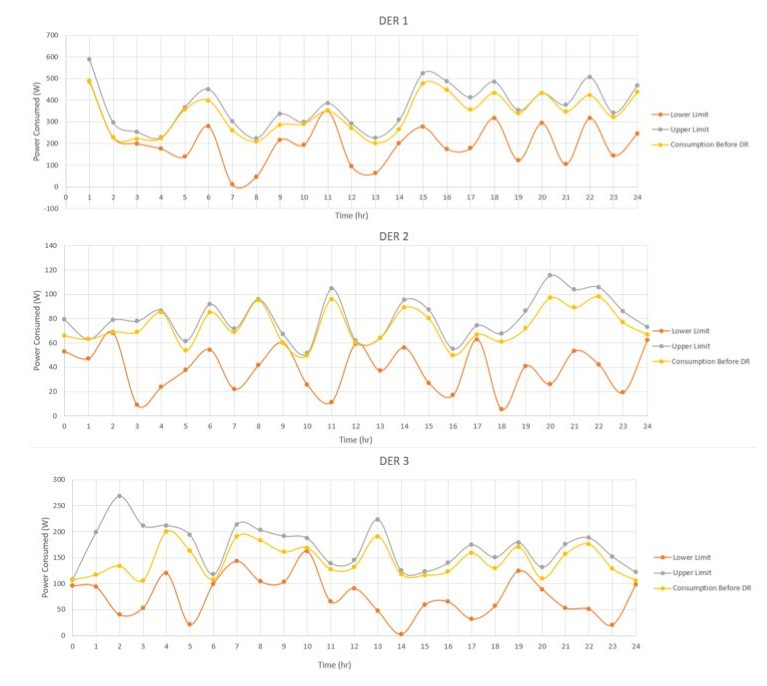
\includegraphics[scale=1]{figures/beforeDR.jpg}
    \caption{Load curves of DR participants before the DR event}
    \label{fig: beforeDR1}
\end{figure}

In Figure \ref{fig: beforeDR1}, the load curves of the 3 DR participants are shown with their upper and lower limits before the DR event.

\begin{figure} [H]
    \centering
    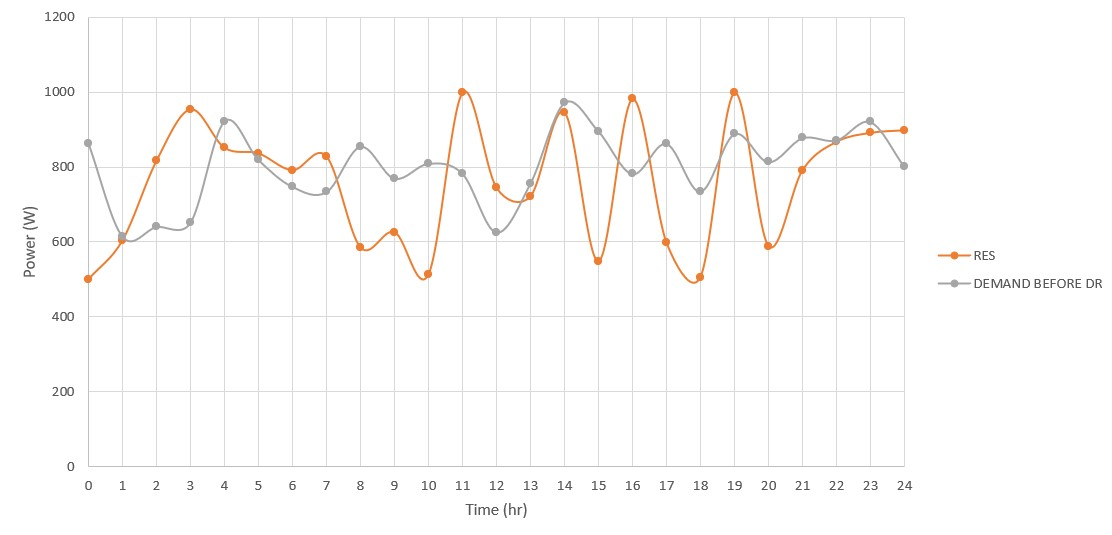
\includegraphics[scale=0.7]{figures/45.jpg}
    \caption{RES output and total demand before DR}
    \label{fig: beforeDR2}
\end{figure}

In Figure \ref{fig: beforeDR2}, the 3 loads are aggregated and compared to the RES generation curve. The computed mean square error is 503,730W. Therefore, a DR event is called to try to reduce the fluctuations.

\begin{figure} [H]
    \centering
    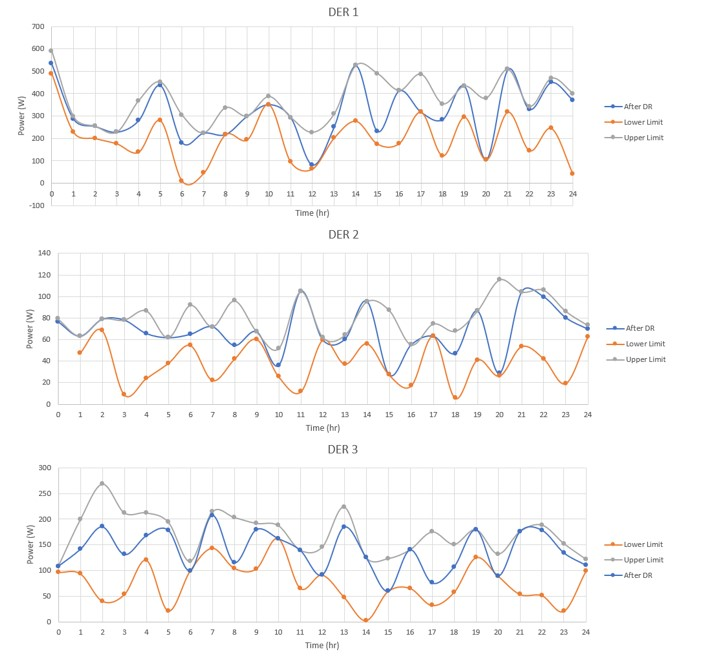
\includegraphics[scale=1.1]{figures/46.jpg}
    \caption{Load curves of DR participants after the DR event}
    \label{fig: beforeDR3}
\end{figure}
For this simulation, the DR participants are assumed to respond ideally while considering their set upper and lower limits. In Figure \ref{fig: beforeDR3},  it can be seen that the responses of the participants are within their upper and lower limits after the DR event.

\begin{figure} [H]
    \centering
    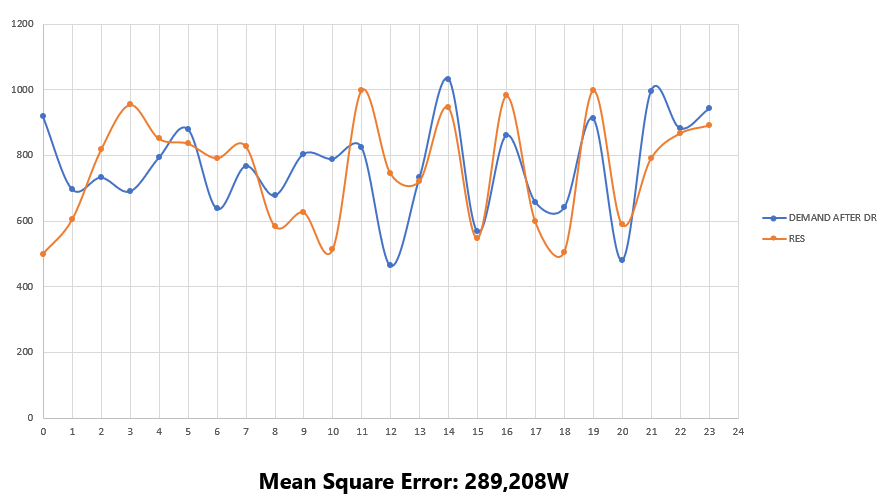
\includegraphics[scale=0.8]{figures/47.png}
    \caption{Total demand after DR event and RES Output}
    \label{fig: beforeDR}
\end{figure}

In Figure \ref{fig: beforeDR}, the three load curves are aggregated and compared with the RES generation curve.  The computed mean square error is 289,208W. Therefore, the DR event reduced the fluctuations.

\begin{figure} [H]
    \centering
    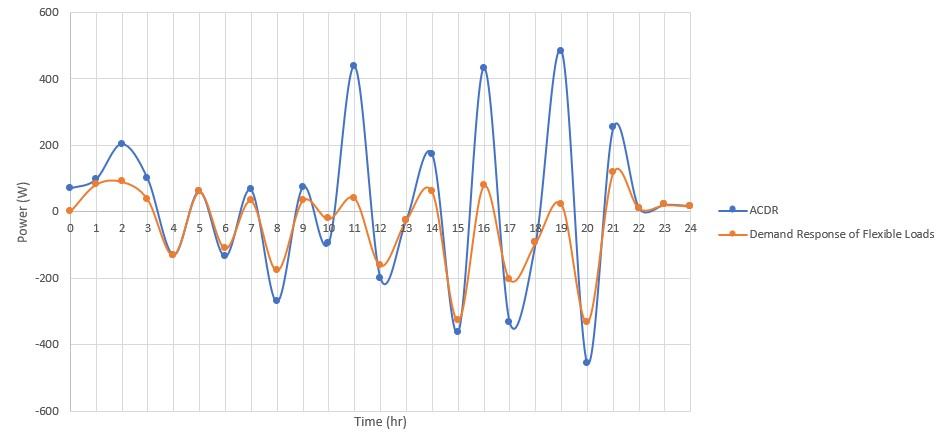
\includegraphics[scale=0.8]{figures/48.jpg}
    \caption{ACDR and Total DR of Flexible Loads}
    \label{fig:ACDR+DR}
\end{figure}

Figure \ref{fig:ACDR+DR} shows the actual demand response and the ACDR. From the result, it can be seen that although the ACDR and DR don't exactly match due to the customer's comfort level limitations, both follow the same trend all throughout the period.

\begin{figure} [H]
    \centering
    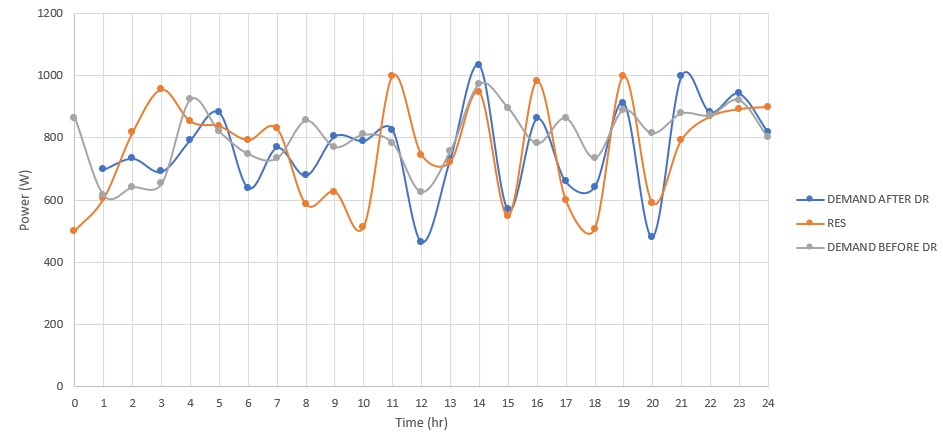
\includegraphics[scale=0.8]{figures/49.jpg}
    \caption{Mean Squared Errors between demand and supply before and after DR}
    \label{fig:MSEs}
\end{figure}

The mean square error of 503,730W was reduced to 289,208W after the demand response events. Shown in Figure \ref{fig:MSEs} is the comparison of the load curves before and after the DR event. In summary, the following are the results of the conducted preliminary simulations:
\begin{itemize}
    \item reduced Mean Square Error
    \item DR followed the ACDR Trend 
    \item minimized fluctuations
\end{itemize}

\chapter{Project Schedule and Deliverables\label{cha:Project-Sked}}
\section{Gantt Chart} \label{sec: Gantt}

Shown in figure \ref{fig:GanttChart} is the proposed timeline of the study spanning 16 weeks. 
https://www.overleaf.com/project/6397325f81f42d1034a859de
\begin{figure} [H]
    \centering
    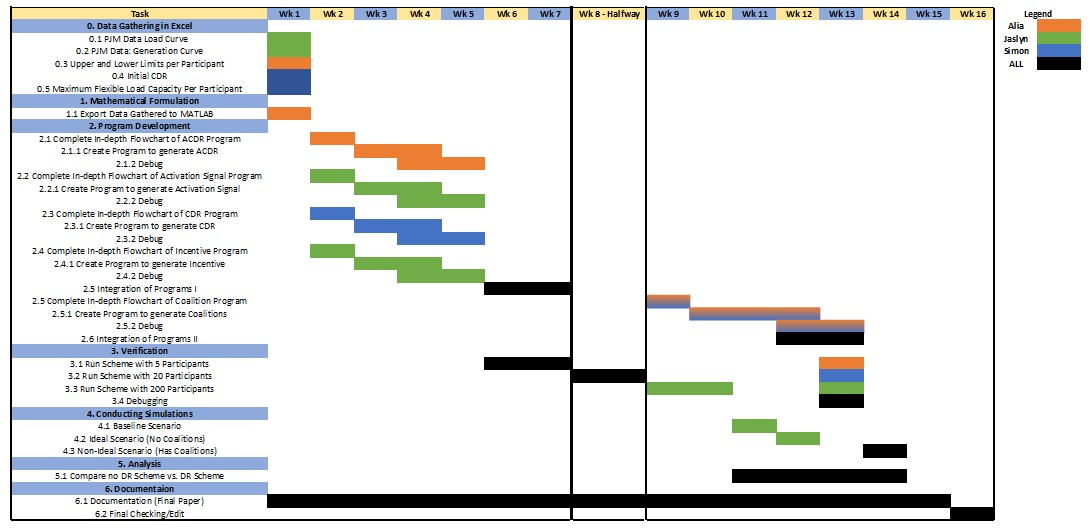
\includegraphics[scale=0.75]{figures/gantt.jpg}
    \caption{Gantt Chart}
    \label{fig:GanttChart}
\end{figure}

The progress updates shall at least have the following sections:

\begin{itemize}
    \item Report summary.
    \item Unforeseen conflicts/problems encountered and how they were solved. 
    \item Accomplished Tasks.
    \item Unaccomplished tasks and plan on how to finish it.
\end{itemize}

\section{Halfway-point Deliverables} \label{sec HPD}

The following tasks listed below should be accomplished by the end of Week 8: 
\begin{itemize}
    \item Programs
    \begin{itemize} 
    \item ACDR Program
    \item Signal Program
    \item CDR Program
    \item Incentive Program
    \item Integration of Programs
     \end{itemize} 
    \item 1st Verification 
    \begin{itemize} 
    \item Run Scheme with 5 Participants
    \item Run Scheme with 20 Participants
    \end{itemize}
    \item Documentation
\end{itemize}

\cleardoublepage{}


\cleardoublepage{}
\printbibliography
\cleardoublepage{}


\end{document}